\chapter{Interferometric methods for tokamak-plasma fluctuations}
\label{ch:InterferometricMethods}
Interferometric methods exploit the interaction of
electromagnetic waves with a plasma
to ascertain properties of the plasma's density.
Because surveying every flavor of interferometric method
exceeds the scope of this work,
only the interferometric methods
of direct relevance to this work ---
external reference-beam interferometry and phase contrast imaging (PCI) ---
are discussed in detail.
Further, the emphasis will be on the diagnosis of
the plasma's density fluctuations rather than its equilibrium density.

Below, Section~\ref{sec:InterferometricMethods:EM_waves_in_plasma}
examines the propagation of electromagnetic waves through a ``cold'' plasma
and derives an expression for the plasma-induced phase delay.
Section~\ref{sec:InterferometricMethods:Gaussian_beam_diffraction} reveals that
plasma-density fluctuations weakly upscatter an downscatter
an incident Gaussian probe beam, while
Section~\ref{sec:InterferometricMethods:imaging} describes
how an imaging system manipulates these scattered beams.
Section~\ref{sec:InterferometricMethods:interferometry} shows that
interfering the imaged probe radiation with an external reference beam
is an effective technique for diagnosing plasma-density fluctuations and
discusses the relative merits of homodyne versus heterodyne detection.
Section~\ref{sec:InterferometricMethods:pci} details the principles of
phase contrast imaging (PCI),
which does away with an external reference beam and
instead applies careful spatial filtering
of the scattered and unscattered beams
to produce its diagnosing interference signal;
further, this section and Appendix~\ref{app:PCIResponseIdentities}
derive the PCI transfer function across the full beam profile, which
is needed to correctly account for PCI's low-$k$ behavior and is,
to the author's knowledge, the first such complete derivation.
Section~\ref{sec:InterferometricMethods:selection}
concludes the chapter by synthesizing the preceding results and
discussing the strengths and limitations of each interferometric technique.


\section{Electromagnetic waves in a plasma}
\label{sec:InterferometricMethods:EM_waves_in_plasma}
A great deal can be learned about a plasma
by probing it with electromagnetic waves.
Sections~\ref{sec:InterferometricMethods:EM_waves_in_plasma:derivation_of_wave_equation}---
\ref{sec:InterferometricMethods:EM_waves_in_plasma:cold_plasma_dispersion_relation}
derive the index of refraction $N$ for a cold, homogeneous plasma.
Section~\ref{sec:InterferometricMethods:EM_waves_in_plasma:propagation_in_inhomogeneous_medium}
extends these results to inhomogeneous plasmas via the WKB approximation and
assesses the validity of this approach for
a CO$_2$ probe beam in a typical tokamak plasma, and
Section~\ref{sec:InterferometricMethods:EM_waves_in_plasma:plasma_induced_phase_delay}
computes the resulting plasma-induced phase delay.


\subsection{Derivation of the wave equation}
\label{sec:InterferometricMethods:EM_waves_in_plasma:derivation_of_wave_equation}
The electric field $\vect{E}$ and the magnetic field $\vect{B}$
of an electromagnetic wave are coupled via Faraday's law
\begin{equation}
  \nabla \cross \vect{E}
  =
  - \frac{\partial \vect{B}}{\partial t}
  \label{eq:InterferometricMethods:Faradays_law}
\end{equation}
and Ampere's law
\begin{equation}
  \nabla \cross \vect{B}
  =
  \mu_0 \vect{J}
  +
  \mu_0 \epsilon_0 \frac{\partial \vect{E}}{\partial t},
  \label{eq:InterferometricMethods:Amperes_law}
\end{equation}
where $\epsilon_0$ is the permittivity of free space,
$\mu_0$ is the permeability of free space, and
$\vect{J}$ is the current density~\cite[Sec.~I.1]{jackson_E&M}.
Note that (\ref{eq:InterferometricMethods:Faradays_law}) and
(\ref{eq:InterferometricMethods:Amperes_law}) are the vacuum formulations
of Faraday's law and Ampere's law;
however, they can still be used to describe
an electromagnetic wave's propagation through a medium
\emph{if} that medium's electromagnetic properties
are explicitly accounted for in the current density $\vect{J}$
\cite[Sec.~I.4]{jackson_E&M}\cite[Sec.~4.1]{hutchinson_diagnostics}.
Now, taking the curl of Faraday's law and
then using Ampere's law to eliminate $\vect{B}$
yields the electric field's wave equation
\begin{equation}
  \nabla^2 \vect{E}
  -
  \frac{1}{c^2} \frac{\partial^2 \vect{E}}{\partial t^2}
  =
  \nabla(\nabla \cdot \vect{E})
  +
  \mu_0 \frac{\partial \vect{J}}{\partial t}.
  \label{eq:InterferometricMethods:wave_equation_pde}
\end{equation}


\subsection{Wave equation in a homogeneous medium}
Fourier decomposing the electric field and the current density
\begin{align}
  \vect{E}(\vect{r}, t)
  &=
  \frac{1}{(2 \pi)^4}
  \int
  \vect{E}(\vect{k}', \omega')
  e^{i(\vect{k}' \cdot \vect{r} - \omega' t)}
  d\vect{k'} \, d\omega',
  \\
  \vect{J}(\vect{r}, t)
  &=
  \frac{1}{(2 \pi)^4}
  \int
  \vect{J}(\vect{k}', \omega')
  e^{i(\vect{k}' \cdot \vect{r} - \omega' t)}
  d\vect{k'} \, d\omega'.
\end{align}
reduces the wave equation (\ref{eq:InterferometricMethods:wave_equation_pde})
to an algebraic equation for each Fourier component.
In particular, for the Fourier mode described by
$\vect{E}_0 e^{i(\vect{k} \cdot \vect{r} - \omega t)}$ and
$\vect{J}_0 e^{i(\vect{k} \cdot \vect{r} - \omega t)}$,
the derivative operators become
$\nabla \rightarrow i \vect{k}$ and
$\partial / \partial t \rightarrow -i \omega$, and
the wave equation reduces to
\begin{equation}
  \left(%
    \vect{N}\vect{N}
    -
    N^2\vect{I}
    +
    \vect{I}
  \right)
  \cdot
  \vect{E}_0
  =
  -\frac{i \vect{J_0}}{\varepsilon_0 \omega},
  \label{eq:InterferometricMethods:wave_equation_algebraic}
\end{equation}
where
\begin{equation}
  \vect{N} \equiv \frac{c \vect{k}}{\omega}
  \label{eq:InterferometricMethods:refraction_index}
\end{equation}
is the index of refraction seen by the given Fourier mode and
$\vect{I}$ is the identity matrix.
Now, assume that the medium is
homogeneous in space and time~\cite[Sec.~3-2]{stix}
such that the current density
is easily related to the electric field via Ohm's law
\begin{equation}
  \vect{J}(\vect{k}, \omega)
  =
  \vect{\sigma}(\vect{k}, \omega)
  \cdot
  \vect{E}(\vect{k}, \omega),
  \label{eq:InterferometricMethods:Ohms_law}
\end{equation}
where $\vect{\sigma}$ is the conductivity of the surrounding medium
\cite[Sec.~I.4]{jackson_E&M}.
Substituting the Ohm's law current density
(\ref{eq:InterferometricMethods:Ohms_law}) into
the Fourier-decomposed wave equation
(\ref{eq:InterferometricMethods:wave_equation_algebraic})
yields the eigenvalue equation
\begin{equation}
  \left[%
    \vect{N}\vect{N}
    -
    N^2\vect{I}
    +
    \left(%
      \vect{I}
      +
      \frac{i \vect{\sigma}}{\varepsilon_0 \omega}
    \right)
  \right]
  \cdot
  \vect{E}_0
  =
  0.
  \label{eq:InterferometricMethods:wave_equation_eigenvalue}
\end{equation}
To proceed further, a model is needed
for the medium's conductivity.


\subsection{The cold-plasma index of refraction}
\label{sec:InterferometricMethods:EM_waves_in_plasma:cold_plasma_dispersion_relation}
Although plasmas in contemporary fusion devices
routinely approach temperatures $\lesssim 100$ million degrees Celsius
($\sim10\times$ the temperature of the core of the sun!),
the thermal velocities of the constituent particles are
still far below the speed of light.
The lightest, and consequently the fastest,
of such a plasma's constituent particles are its electrons,
which have thermal velocities $\lesssim 0.1 c$.
In contrast, as will be shown shortly,
the electromagnetic waves used to make interferometric measurements
in such plasmas have phase velocities very close to the speed of light.
Thus, in the context of the wave-plasma interaction,
the unperturbed plasma can be modeled as a collection
of motionless (i.e.\ zero-temperature or ``cold'') charged particles.
Consequently, the pressure of this model plasma is zero.
For the present application, it is also appropriate
to neglect the perturbed motion of the ions,
whose inertia greatly exceeds that of the electrons, and
to neglect collisions,
which are relatively rare in fusion plasmas.
The electron-fluid momentum equation for such a plasma is
\begin{equation}
  m_e n_e \frac{d \vect{v}_e}{dt}
  =
  -e n_e \left( \vect{E} + \vect{v}_e \cross \vect{B} \right),
  \label{eq:InterferometricMethods:cold_plasma_momentum_equation}
\end{equation}
where $n_e$ is the electron density,
$\vect{v}_e$ is the perturbed electron-fluid velocity, and
$d/dt = \partial / \partial t + (\vect{v}_e \cdot \nabla)$
is the advective time derivative.
Linearizing and Fourier analyzing
the electron-fluid momentum equation
(\ref{eq:InterferometricMethods:cold_plasma_momentum_equation})
yields
\begin{equation}
  i \omega m_e \vect{v}_e
  =
  e \left( \vect{E} + \vect{v}_e \cross \vect{B}_0 \right),
  \label{eq:InterferometricMethods:cold_plasma_momentum_equation_linear_and_Fourier}
\end{equation}
where $\vect{B}_0$ is the equilibrium magnetic field.
Let $\vect{B}_0 = B_0 \hat{\vect{z}}$.
Then, the perturbed electron-fluid velocity $\vect{v}_e$
is easily found to be~\cite[Sec.~4.1.2]{hutchinson_diagnostics}
\begin{align}
  v_{e,x}
  &=
  \frac{-i e}{\omega m_e}
  \frac{1}{1 - \Omega_e^2 / \omega^2}
  \left( E_x - i \frac{\Omega_e}{\omega} E_y \right),
  \\
  v_{e,y}
  &=
  \frac{- i e}{\omega m_e}
  \frac{1}{1 - \Omega_e^2 / \omega^2}
  \left( i \frac{\Omega_e}{\omega} E_x + E_y \right),
  \\
  v_{e,z}
  &=
  \frac{- i e}{\omega m_e} E_z,
\end{align}
where
\begin{equation}
  \Omega_e \equiv \frac{e B_0}{m_e}
  \label{eq:InterferometricMethods:cyclotron_frequency_electron}
\end{equation}
is the electron cyclotron frequency.
Having neglected the ion's motion,
the current density is simply
\begin{equation}
  \vect{J} = -e n_e \vect{v}_e.
  \label{eq:InterferometricMethods:current_density_electron_motion}
\end{equation}
Equating the current densities from
(\ref{eq:InterferometricMethods:Ohms_law}) and
(\ref{eq:InterferometricMethods:current_density_electron_motion})
and substituting the solution for $\vect{v}_e$ yields
the plasma's conductivity~\cite[Sec.~4.1.2]{hutchinson_diagnostics}
\begin{equation}
  \vect{\sigma}
  =
  \frac{i n_e e^2}{m_e \omega}
  \frac{1}{1 - \Omega_e^2 / \omega^2}
  \begin{pmatrix}
    1                   & -i \Omega_e / \omega & 0
    \\
    i \Omega_e / \omega &  1                   & 0
    \\
    0                   & 0                    & 1 - \Omega_e^2 / \omega^2
  \end{pmatrix}.
  \label{eq:InterferometricMethods:cold_plasma_conductivity}
\end{equation}
Choose axes such that
\begin{equation}
  \vect{k} = k ( \sin\theta \hat{\vect{y}} + \cos\theta \hat{\vect{z}} ).
  \label{eq:InterferometricMethods:wavevector_in_convenient_basis}
\end{equation}
Then, substituting the cold-plasma conductivity
(\ref{eq:InterferometricMethods:cold_plasma_conductivity})
into the electric field's eigenvalue equation
(\ref{eq:InterferometricMethods:wave_equation_eigenvalue})
and solving for the corresponding eigenvalues yields
the well-known Appleton-Hartree formula
for the plasma's index of refraction
\cite[Sec.~4.1.2]{hutchinson_diagnostics}
\begin{equation}
  N^2
  =
  1
  -
  \frac{X (1 - X)}{ 1 - X - \frac{1}{2} Y^2 \sin^2 \theta \pm \Delta },
  \label{eq:InterferometricMethods:Appleton_Hartree}
\end{equation}
where
\begin{align}
  X &\equiv \frac{\omega_{pe}^2}{\omega^2},
  \label{eq:InterferometricMethods:X}
  \\
  Y &\equiv \frac{\Omega_e}{\omega},
  \label{eq:InterferometricMethods:Y}
  \\
  \Delta
  &=
  \left[
    \left( \frac{1}{2} Y^2 \sin^2\theta \right)^2
    +
    (1 - X)^2 Y^2 \cos^2\theta
  \right]^{1/2},
  \\
  \omega_{pe}^2 &\equiv \frac{n_e e^2}{m_e \varepsilon_0};
  \label{eq:InterferometricMethods:angular_electron_plasma_frequency}
\end{align}
here, $\omega_{pe}$ is referred to as the angular electron plasma frequency.

The refractive index formula
can be dramatically simplified
for high-frequency electromagnetic waves
propagating in typical tokamak plasmas.
For example, a CO$_2$ beam ($\omega = 2 \pi \cdot \SI{28.3}{\tera\hertz}$)
propagating in a typical \diiid\space plasma sees
\begin{align}
  n_e
  \lesssim
  \SI{e20}{\per\meter\cubed}
  \qquad
  &\Rightarrow
  \qquad
  X \lesssim 10^{-5},
  \notag \\
  B
  \lesssim
  \SI{2}{\tesla}
  \qquad
  &\Rightarrow
  \qquad
  Y \lesssim 2 \times 10^{-3}.
  \notag
\end{align}
Now, the smallness of $X$ and $Y$ can be exploited
to approximate the Appleton-Hartree index of refraction
(\ref{eq:InterferometricMethods:Appleton_Hartree})
by retaining only the terms that are linear in $X$ or linear in $Y$;
this yields $N^2 \approx 1 - X$ or, equivalently,
\begin{equation}
  N \approx 1 - \frac{X}{2}.
  \label{eq:InterferometricMethods:index_of_refraction}
\end{equation}
Note that the corresponding phase velocity is
$v_{\text{ph}} = c / N \approx c$.
Thus, the cold-plasma assumption that the wave's phase velocity
is much larger than the thermal velocities ($\lesssim 0.1 c$)
of the plasma's constituent particles is valid.

It is enlightening to also examine
the corresponding electric-field eigenvectors.
Substituting the index of refraction
(\ref{eq:InterferometricMethods:index_of_refraction})
into the corresponding eigenvalue equation
(\ref{eq:InterferometricMethods:wave_equation_eigenvalue}) and
solving to lowest order for the corresponding eigenvector yields
\begin{equation}
  \vect{E}_0
  \approx
  E_{0,x} \hat{\vect{x}}
  +
  E_{0,yz} (\hat{\vect{k}} \cross \hat{\vect{x}}),
  \label{eq:InterferometricMethods:electric_field_eigenvector}
\end{equation}
where $\hat{\vect{k}} = \vect{k} / |\vect{k}|$
is the unit vector corresponing to the wavector defined in
(\ref{eq:InterferometricMethods:wavevector_in_convenient_basis}), and
$E_{0,x}$ and $E_{0,yz}$ are arbitrary, uncoupled constants
that are independent of the plasma's properties.
Thus, to lowest order, a CO$_2$ beam in a tokamak plasma
propagates as a transverse electromagnetic wave
($\vect{k} \cdot \vect{E}_0 \approx 0$)
with near-constant polarization.

Finally, it should be noted for completeness that
while cold-plasma theory is adequate for the current purposes,
finite-temperature and relativistic effects
will affect the interpretation of refractive index measurements
in a fusion reactor.
For example, the thermal correction
to the cold-plasma interferometric phase
in a $T_e \approx 10 \, \text{keV}$ plasma is $-3\%$,
with slightly more substantial corrections for
polarimetric measurements~\cite{mirnov_07}.


\subsection{Wave propagation in an inhomogeneous medium}
\label{sec:InterferometricMethods:EM_waves_in_plasma:propagation_in_inhomogeneous_medium}
No physical plasma is truly homogeneous in space.
While the above Fourier approach can still be employed,
the inhomogeneities tend to couple the various modes together,
greatly complicating the analysis.
However, if the plasma varies sufficiently slowly,
the plasma can be treated as \emph{locally} uniform, and
the wave field can be ``stitched'' together
as the wave propagates from initial position $\vect{r}^{(i)}$
to position $\vect{r}$ via the WKB approximation
\cite[Ch.~13]{stix}\cite[Ch.~8]{griffiths_QM}
\begin{equation}
  E(\vect{r}, t)
  \approx
  E_0 \exp \left[i \left(%
    \int_{\vect{r}^{(i)}}^{\vect{r}} \vect{k}(\vect{r}') \cdot d\vect{l}'
    -
    \omega t
  \right) \right].
  \label{eq:InterferometricMethods:WKB_field}
\end{equation}
Here, $\vect{k}(\vect{r}')$ is the local wavevector and
the integration is performed along the wave's trajectory.
Note that the amplitude variation and the reflected wave
that are characteristic of the WKB approximation
have been neglected because densities in a tokamak plasma
are much less than a CO$_2$ beam's
$\sim \SI{e25}{\per\meter\cubed}$ density cutoff.

What exactly is meant by ``sufficiently slowly'', though?
To approximate the plasma as locally uniform,
the change in the wavenumber $\delta k$ over one wavelength $\lambda$
should be small relative to the wavenumber $k$.
Note that the change in wavenumber over one wavelength is
$\delta k = \nabla k \cdot \lambda = 2 \pi \nabla k / k$.
Thus, the WKB validity criterion that $\delta k / k \ll 1$ becomes
\begin{equation}
  \frac{|\nabla k|}{k^2} \ll \frac{1}{2 \pi}.
  \label{eq:InterferometricMethods:WKB_validity}
\end{equation}
Now, using the definition of $N$ from
(\ref{eq:InterferometricMethods:refraction_index}),
the cold-plasma index of refraction in
(\ref{eq:InterferometricMethods:index_of_refraction})
can be rewritten as $k = (\omega / c) (1 - X / 2)$, and, to lowest order,
\begin{equation}
  \nabla k
  \approx
  -\left( \frac{2 \pi \, r_e}{k} \right) \nabla n_e,
\end{equation}
where
\begin{equation}
  r_e
  =
  \frac{e^2}{4 \pi \varepsilon_0 m_e c^2}
  =
  \SI{2.8e-15}{\meter}
  \label{eq:InterferometricMethods:classical_electron_radius}
\end{equation}
is the classical electron radius.
The most extreme density gradients in a tokamak
often occur in the so-called ``pedestal'',
where the density changes by
$\Delta n_e \lesssim \SI{e20}{\per\meter\cubed}$
over a scale length $\Delta r \gtrsim \SI{1}{\centi\meter}$;
for a CO$_2$ laser beam ($k = \SI{5.9e5}{\per\meter}$)
propagating through such a pedestal,
\begin{equation}
  \frac{|\nabla k|}{k^2}
  =
  \left( \frac{2 \pi \, r_e}{k^3} \right) |\nabla n_e|
  \lesssim
  10^{-9}
  \notag
\end{equation}
such that the criterion for WKB validity
(\ref{eq:InterferometricMethods:WKB_validity})
is very well-satisfied.
The WKB validity criterion can also be evaluated
for a CO$_2$ beam propagating through plasma-density fluctuations;
assuming $\tilde{n}_e / \bar{n}_e \sim 10^{-3}$,
$\bar{n}_e \lesssim \SI{e20}{\per\meter\cubed}$, and
density-fluctuation wavenumbers $\lesssim \SI{30}{\per\centi\meter}$,
$|\nabla k| / k^2 \lesssim 2 \times 10^{-11}$ such that
the WKB validity criterion is also very well-satisfied
for typical plasma-density fluctuations.


\subsection{Plasma-induced phase delay}
\label{sec:InterferometricMethods:EM_waves_in_plasma:plasma_induced_phase_delay}
The WKB field solution (\ref{eq:InterferometricMethods:WKB_field})
indicates that the wave's phase at a given point in space and time
is determined by the properties of the medium
that the wave has passed through.
In particular, a CO$_2$ laser beam propagating through a tokamak plasma
will acquire a phase shift $\phi$ relative to vacuum given by
\begin{align}
  \phi
  &=
  \int \left[ k(\vect{r}) - \frac{\omega}{c} \right] dl
  \notag \\
  &=
  \frac{\omega}{c} \int \left[ N(\vect{r}) - 1 \right] dl
  \notag \\
  &\approx
  \frac{\omega}{c}
  \int \left[%
    \left( 1 - \frac{X}{2} \right) - 1
  \right] dl
  \notag \\
  &=
  -r_e \lambda_0 \int n_e dl,
  \label{eq:InterferometricMethods:phase}
\end{align}
where the index of refraction has been approximated via
(\ref{eq:InterferometricMethods:index_of_refraction}),
$\lambda_0 = 2 \pi c / \omega = \SI{10.6}{\micro\meter}$
is the CO$_2$ beam's vacuum wavelength, and
$r_e$ is again the classical electron radius
defined in (\ref{eq:InterferometricMethods:classical_electron_radius}).
Now, if the plasma fluctuates about its equilibrium density $\bar{n}_e$ as
$n_e = \bar{n}_e + \tilde{n}_e$,
the phase will similarly fluctuate about its equilibrium as
$\phi = \bar{\phi} + \tilde{\phi}$ where
\begin{equation}
  \tilde{\phi}
  =
  - r_e \lambda_0 \int \tilde{n}_e dl.
  \label{eq:InterferometricMethods:phase_fluctuation}
\end{equation}
It is precisely the intent of
Section~\ref{sec:InterferometricMethods:Gaussian_beam_diffraction}
to determine how such density fluctuations
interact with an incident Gaussian probe beam.
As a final note before leaving this section,
accurate interpretation of very rapid phase-fluctuation measurements
(such as those resulting from RF-wave perturbations)
may require accounting for the beam's finite transit time
through the plasma to the point of measurement
\cite[Sec.~3.1]{tsujii_phd}.


\section{Diffraction of a Gaussian probe beam}
\label{sec:InterferometricMethods:Gaussian_beam_diffraction}
Lasers are almost always well-collimated enough that
they are amenable to analysis in the paraxial limit.
Gaussian beams are exact solutions
to the paraxial wave equation in free space, and
they are very good approximations
to the eigenmodes observed in real lasers~\cite[Ch.~16]{siegman_lasers}.
For this reason, it is reasonable to investigate
the interaction of a Gaussian probe beam
with a plasma-density fluctuation.


\subsection{Definition of a Gaussian beam}
\label{sec:InterferometricMethods:Gaussian_beam_diffraction:Gaussian_beam_definition}
A Gaussian beam of angular frequency $\omega_0$
propagating along the $z$-axis
in a medium with index of refraction $N$
has an electric field
\begin{equation}
  E_G(\vect{r}, t)
  =
  E_G(\vect{r}) e^{-i \omega_0 t}
\end{equation}
with spatial dependence~\cite[Ch.~17]{siegman_lasers}
\begin{equation}
  \begin{aligned}
    E_G(\vect{r})
    &=
    E_0
    \frac{w_0}{w(z)}
    \exp\left[ \frac{-\rho^2}{w(z)^2} \right]
    \\
    &\quad\times
    \exp\left\{ i \left[
      N k_0 z
      +
      \frac{N k_0 \rho^2}{2 R(z)}
      -
      \psi(z) \right] \right\}.
  \end{aligned}
  \label{eq:InterferometricMethods:Gaussian_beam}
\end{equation}
Here,
$\rho = (x^2 + y^2)^{1/2}$ is the transverse distance
from the $z$-axis (i.e.\ the beam's ``symmetry axis''),
$w_0$ is the radius of the beam's waist, and
$k_0 = \omega_0 / c = 2 \pi / \lambda_0$
is the beam's vacuum wavenumber.
The beam's width $w(z)$, radius of curvature $R(z)$, and
Gouy phase $\psi(z)$ are defined as
\begin{align}
  w(z)
  &=
  w_0 \left[ 1 + \left( \frac{z}{z_R} \right)^2 \right]^{1/2},
  \label{eq:InterferometricMethods:Gaussian_beam_width}
  \\
  R(z)
  &=
  z \left[ 1 + \left( \frac{z_R}{z} \right)^2 \right],
  \label{eq:InterferometricMethods:Gaussian_beam_radius_of_curvature}
  \\
  \psi(z)
  &=
  \atan\left( \frac{z}{z_R} \right),
  \label{eq:InterferometricMethods:Gouy_phase}
\end{align}
where the Rayleigh range
\begin{equation}
  z_R \equiv \left( \frac{\pi w_0^2}{\lambda_0} \right) N
  \label{eq:InterferometricMethods:Rayleigh_range}
\end{equation}
is the nominal division between the beam's
near-field ($|z| \ll z_R$) and far-field ($|z| \gg z_R$) behaviors.
Note that the beam's waist sits at $z = 0$.

From a Fourier perspective,
a Gaussian beam can be decomposed into a set of infinite plane waves
traveling in slightly different directions \cite[Ch.~16.7]{siegman_lasers}.
The plane waves with the beam's nominal wavevector
$\vect{k}_0 = k_0 \hat{\vect{z}}$
propagate along the beam's symmetry axis, while
the plane waves with non-zero transverse wavevectors
produce beam divergence (i.e.\ free-space diffraction of the beam).
This behavior can be understood as an uncertainty principle, with
the beam's finite transverse dimensions
necessarily requiring a finite spread in transverse wavevectors.


\subsection{Diffraction of a Gaussian beam from plasma-density fluctuations}
\label{sec:InterferometricMethods:Gaussian_beam_diffraction:from_plasma_density_fluctuations}
As discussed in the text surrounding
(\ref{eq:InterferometricMethods:electric_field_eigenvector}),
a CO$_2$ probe beam in a tokamak plasma propagates
as a transverse electromagnetic wave with near-constant polarization
(any small changes to the beam polarization
are of little practical interest to the present work).
Thus, a \emph{scalar} diffraction theory is sufficient
to describe the relevant aspects of the beam-plasma interaction;
the details of this theory are provided in
Appendix~\ref{app:GaussianBeamDiffraction}, and
the relevant results are summarized below.

A Gaussian CO$_2$ probe beam
propagating through a tokamak plasma
acquires a plasma-induced phase delay $\phi(\vect{\rho}', t)$
given by (\ref{eq:InterferometricMethods:phase}),
where $\vect{\rho}'$ corresponds to the beam's transverse dimensions.
Explicitly dividing $\phi$ into bulk $\bar{\phi}(t)$ and
spatially varying $\tilde{\phi}(\vect{\rho}', t)$ components,
the plasma-induced phase delay becomes
\begin{equation}
  \phi(\vect{\rho}', t) = \bar{\phi}(t) + \tilde{\phi}(\vect{\rho}', t).
\end{equation}
Typically, $\tilde{\phi}$ varies on much faster time scales than $\bar{\phi}$,
but this is not required.
The spatial variation of the plasma-induced phase delay
contributes to the diffraction of the incident Gaussian probe beam.

The response functions of the diagnostics investigated in
Sections~\ref{sec:InterferometricMethods:interferometry} and
\ref{sec:InterferometricMethods:pci} will be shown
to be linear in their regimes of relevance, so
it is sufficient to examine diffraction
from phase fluctuations $\tilde{\phi}$
consisting of a single Fourier mode
\begin{equation}
  \tilde{\phi}(\vect{\rho}', t) = \tilde{\phi}_0 \cos(k x' - \omega t).
  \label{eq:InterferometricMethods:cosine_phase_fluctuation}
\end{equation}
Here, without loss of generality,
it is assumed that the CO$_2$ probe beam
is propagating in the $+z$-direction, and
the density fluctuation corresponding to $\tilde{\phi}$
is propagating in the $x$-direction.
Then, following the formalism pioneered by Raman and Nath
\cite{raman_nath_diffraction_partI,raman_nath_diffraction_partIII} and
detailed in Appendix~\ref{app:GaussianBeamDiffraction},
the diffracted electric field can be written
(see (\ref{eq:GaussianBeamDiffraction:phase_modulated_Gaussian_beam_diffraction}))
as a discrete sum of scattered beams
\begin{equation}
  E(\vect{r}, t)
  \approx
  e^{i \bar{\phi}}
  \sum_{m = -1}^{1}
  i^m \left[ J_m(\tilde{\phi}_0) \right]
  E_G(\vect{r}_m)
  e^{-i (\omega_0 + m \omega) t},
  \label{eq:InterferometricMethods:phase_modulated_Gaussian_beam_diffraction}
\end{equation}
where
$J_m$ is the $m$\ts{th} Bessel function of the first kind and
$E_G(\vect{r}_m)$ is the spatial dependence of the $m$\ts{th} scattered beam.
Note that $\vect{r}_m = [ \vect{R}(\theta_m) ] \vect{r}$
is the native coordinate system
of the $m$\ts{th} scattered beam
expressed in lab-frame coordinates;
here, $\theta_m \approx mk / k_0$ is the angle
at which the $m$\ts{th} scattered beam propagates
relative to the lab-frame optical axis, and
\begin{equation}
  \vect{R}(\theta)
  =
  \begin{pmatrix}
    \cos\theta & 0 & -\sin\theta
    \\
    0          & 1 & 0
    \\
    \sin\theta & 0 & \cos\theta
  \end{pmatrix}
  \label{eq:InterferometricMethods:rotation_matrix}
\end{equation}
is the rotation matrix
that rotates the $(x, z)$-plane about the $y$-axis by angle $\theta$.

It is worth pausing to discuss the physical significance
of the diffracted electric field
(\ref{eq:InterferometricMethods:phase_modulated_Gaussian_beam_diffraction}).
The assumed sinusoidal phase modulation
(\ref{eq:InterferometricMethods:cosine_phase_fluctuation})
diffracts an incident Gaussian beam
predominantly into downscattered ($m = -1$), unscattered ($m = 0$), and
upscattered ($m = 1$) Gaussian beams.
The incident beam is coupled into the $m$\ts{th} scattered beam
with strength $J_m(\tilde{\phi}_0)$.
The $m$\ts{th} scattered beam is Doppler shifted
relative to the incident beam by $m \omega$ and
propagates at an angle $\theta_m \approx m k / k_0$
relative to the lab-frame optical axis.
The scattering is very nearly elastic
(i.e.\
$\omega / \omega_0
\lesssim
\SI{1}{\giga\hertz} / \SI{28.3}{\tera\hertz}
\sim 10^{-5}$), so
$|\vect{k}_{0,m}| = k_0$ is a very good approximation.
This constraint of elasticity
coupled with knowledge of the scattering angle $\theta_m$
allows determination of the scattered wavevector
\begin{equation}
  \vect{k}_{0,m}
  =
  (m k) \hat{\vect{x}}
  +
  k_0 \left[ 1 - \left(\frac{m k}{k_0}\right)^2 \right]^{1/2} \hat{\vect{z}}.
  %k_0 \sqrt{1 - \left(\frac{m k}{k_0}\right)^2} \hat{\vect{z}}
  \label{eq:InterferometricMethods:scattered_beam_wavevector}
\end{equation}
Finally, note that the simultaneous presence
of both the upscattered and downscattered beams
(a key prediction of the Raman-Nath formalism)
under typical experimental conditions
has been demonstrated empirically
\cite[Sec.~2.1]{dorris_phd}.


\subsection{Wavenumber filtering of the diffracted field}
Some interferometric techniques, such as phase contrast imaging
(PCI; discussed in Section~\ref{sec:InterferometricMethods:pci}),
filter the Fourier wavenumber content
of the diffracted electric field
(\ref{eq:InterferometricMethods:phase_modulated_Gaussian_beam_diffraction}).
The mathematical formalism for such filtering is detailed in
Appendix~\ref{app:GaussianBeamDiffraction}, but
the relevant results are briefly summarized here.
Assume that the filtering can be described by a transfer function $T(k_x)$,
where $k_x$ is the wavevector component in the lab-frame $x$-direction.
Then, the filtered electric field can be written
(see (\ref{eq:GaussianBeamDiffraction:phase_modulated_Gaussian_beam_diffraction_Fourier_filtered}))
as
\begin{equation}
  E(\vect{r}, t)
  \approx
  e^{i \bar{\phi}}
  \sum_{m = -1}^{1}
  i^m \left[ J_m(\tilde{\phi}_0) \right]
  E_T(\vect{r}_m)
  e^{-i (\omega_0 + m \omega) t},
  \label{eq:InterferometricMethods:phase_modulated_Gaussian_beam_diffraction_Fourier_filtered}
\end{equation}
where
\begin{equation}
  E_T(\vect{r}_m)
  \approx
  E_G(0, y_m, z_m)
  \cdot
  \mathcal{E}(\vect{r}_m, k),
  \label{eq:InterferometricMethods:mth_diffracted_beam_kx_filtered_compact}
\end{equation}
is the $m$\ts{th} scattered beam
following the wavenumber-filtering transformation, and
\begin{equation}
  \begin{aligned}
    \mathcal{E}(\vect{r}_m, k)
    &=
    \frac{e^{-i m k x_m}}{2 \pi}
    \\
    &\quad \times
    \int dx' \,
    \exp\left[ \frac{-x'^2}{w(z_m)^2} \right]
    \exp\left\{%
      i \left[%
        m k x'
        +
        \frac{k_0 x'^2}{2 R(z_m)}
      \right]
    \right\}
    \\
    &\quad \times
    \int dk_x \,
    T(k_x)
    e^{i k_x (x_m - x')}
  \end{aligned}
  \label{eq:InterferometricMethods:mth_diffracted_beam_kx_filtered_transformation}
\end{equation}
is a complex-valued function
that describes the amplitude and phase transformations
that result from filtering the $m$\ts{th} scattered beam by $T(k_x)$.
When there is no wavenumber filtering (i.e. $T(k_x) = 1$),
the $m$\ts{th} transformed beam
(\ref{eq:InterferometricMethods:mth_diffracted_beam_kx_filtered_compact})
readily reduces to the $m$\ts{th} scattered Gaussian beam
(i.e.\ $E_T(\vect{r}_m) = E_G(\vect{r}_m)$),
in agreement with expectations.


\section{Imaging of the diffracted field}
\label{sec:InterferometricMethods:imaging}
It is often desirable to \emph{image} the above diffracted field
in order to determine the spatiotemporal aspects
of the responsible phase fluctuations.
Below, the relevant aspects of imaging systems are briefly reviewed.
The imaged field is then computed and
examined under typical experimental limits.


\subsection{Imaging systems}
Appendix~\ref{app:ImagingSystems} details
the geometric optics and Gaussian-beam transformations
of relevance to imaging systems;
here, the directly applicable aspects
are briefly summarized.

Let the optical axis of an arbitrary optical system lie along the $z$-axis,
and let all optical rays lie in a plane with the optical axis.
At a given position $z_j$, an optical ray is fully described by
its transverse distance $\rho$ to the optical axis and
its slope $d\rho / dz$~\cite[Ch.~15]{siegman_lasers}.
An imaging system $\image$, by definition,
redirects all rays emanating from transverse position $\rho_{\object}$
in the object plane $S_{\object}$
to intersect at transverse position
\begin{equation}
  \rho_{\image} = M \rho_{\object}
  \label{eq:InterferometricMethods:image_plane_transverse_coordinates}
\end{equation}
in the image plane $S_{\image}$.
Here, $M$ is the \emph{magnification} of the imaging system, and
$M < 0$ implies that the image is inverted relative to the object.
Because the symmetry axis of a Gaussian beam
behaves as a ray in the geometric-optics sense
\cite{tovar_generalized_beam_matrices_IV},
the symmetry axes of the unscattered and scattered beams
intersect in the image plane.
Then, varying inversely with the spatial scale,
the wavenumber $k$ of the object-plane phase fluctuation
(\ref{eq:InterferometricMethods:cosine_phase_fluctuation})
is imaged as
\begin{equation}
  k_{\image} \equiv \frac{k}{M}.
  \label{eq:InterferometricMethods:image_plane_fluctuation_wavenumber}
\end{equation}
The native coordinate systems
of the $m$\ts{th} scattered beam and the unscattered beam
do \emph{not} align in the image plane
(i.e.\ $\vect{r}_{m,\image} \neq \vect{r}_{\image}$).
Considerations from geometric and Gaussian-beam optics
show that the image-plane coordinate systems are related as
\begin{equation}
  \begin{pmatrix}
    x_{m, \image}
    \\
    y_{m, \image}
    \\
    z_{m, \image}
  \end{pmatrix}
  =
  \begin{pmatrix}
    x_{\image} \cos\left( \frac{\theta_m}{M} \right)
    \\
    y_{\image}
    \\
    z_{\image} + x_{\image} \sin\left( \frac{\theta_m}{M} \right)
  \end{pmatrix}
  \approx
  \begin{pmatrix}
    x_{\image}
    \\
    y_{\image}
    \\
    z_{\image} + x_{\image} \left( \frac{\theta_m}{M} \right)
  \end{pmatrix},
  \label{eq:InterferometricMethods:coordinate_transformation_imaging_plane}
\end{equation}
where the approximation is valid to first order in $\theta_m / M$.


\subsection{The imaged field}
Let $\image$ image the object plane $S_{\object}$
such that the diffracted field
(\ref{eq:InterferometricMethods:phase_modulated_Gaussian_beam_diffraction_Fourier_filtered})
is imaged as
\begin{align}
  E(\vect{r}_{\image}, t)
  &=
  \image[ E(\vect{r}_{\object}, t) ]
  \notag \\
  &\begin{aligned}
    =
    e^{i \bar{\phi}}
    \sum_{m = -1}^{1}
    \biggl\{%
      &i^m \left[ J_m(\tilde{\phi}_0) \right]
      \\
      &\times
      \image[E_T(\vect{r}_{m, \object})]
      e^{-i (\omega_0 + m \omega) t}
    \biggr\},
  \end{aligned}
  \label{eq:InterferometricMethods:imaged_total_field_v1}
\end{align}
where the $\image$ operator has been brought within the summation
because the scattered beams obey the superposition principle
when propagating through the imaging system
(it is assumed that typical beam intensities are far from
any nonlinear thresholds in the imaging-system materials).
The effect of $\image$ is to propagate each scattered beam
from its object-plane coordinates $\vect{r}_{m, \object}$
to its corresponding image-plane coordinates $\vect{r}_{m, \image}$.
Thus, referencing the definition of $E_T(\vect{r}_{m})$ in
(\ref{eq:InterferometricMethods:mth_diffracted_beam_kx_filtered_compact}),
it readily follows that
\begin{align}
  \image[E_T(\vect{r}_{m, \object})]
  &=
  \mathcal{I}[%
    E_G(0, y_{m, \object}, z_{m, \object})
    \cdot
    \mathcal{E}(\vect{r}_{m, \object}, k)
  ]
  \notag \\
  &=
  E_G(0, y_{m, \image}, z_{m, \image})
  \cdot
  \mathcal{E}(\vect{r}_{m, \image}, k_{\image})
  \notag \\
  &\approx
  E_G(0, y_{\image}, z_{\image})
  e^{i m k_{\image} x_{\image}}
  \cdot
  \mathcal{E}(\vect{r}_{m, \image}, k_{\image}),
\end{align}
where the last step naturally follows from
the image-plane coordinate transformation
(\ref{eq:InterferometricMethods:coordinate_transformation_imaging_plane})
and the following approximations:
$w(z_{m, \image}) \approx w(z_{\image})$,
$R(z_{m, \image}) \approx R(z_{\image})$, and
$\psi(z_{m, \image}) \approx \psi(z_{\image})$.
Thus, the imaged field
(\ref{eq:InterferometricMethods:imaged_total_field_v1}) becomes
\begin{equation}
  \begin{aligned}
    E(\vect{r}_{\image}, t)
    &=
    E_G(0, y_{\image}, z_{\image}, t)
    e^{i \bar{\phi}}
    \\
    &\quad \times
    \sum_{m = -1}^{1}
    i^m \left[ J_m(\tilde{\phi}_0) \right]
    \mathcal{E}(\vect{r}_{m, \image}, k_{\image})
    e^{i m \nu},
  \end{aligned}
  \label{eq:InterferometricMethods:imaged_total_field}
\end{equation}
where
\begin{equation}
  \nu
  =
  k_{\image} x_{\image} - \omega t
  \label{eq:InterferometricMethods:image_plane_nu}
\end{equation}
and
$E_G(0, y_{\image}, z_{\image}, t)
=
E_G(0, y_{\image}, z_{\image}) e^{-i \omega_0 t}$.


\subsection{The weak-coupling limit}
\label{sec:InterferometricMethods:imaging:weak_coupling_limit}
Typically, the phase-fluctuation amplitude
is very small ($\tilde{\phi}_0 \ll 1$), and
the Bessel function's small-argument limiting form \cite{abramowitz_and_stegun}
can be used
\begin{equation}
  \lim_{z \rightarrow 0} J_m(z)
  \sim
  \begin{cases}
    \frac{1}{\Gamma(m + 1)} \left( \frac{z}{2} \right)^m
    , \qquad
    &m = 0, 1, 2, 3, \cdots,
    \\
    \frac{1}{\Gamma(|m| + 1)} \left( \frac{-z}{2} \right)^{|m|}
    , \qquad
    &m = -1, -2, -3, \cdots.
  \end{cases}
\end{equation}
Here, $\Gamma$ is the gamma function, and
$\Gamma(m + 1) = m!$ for positive integer $m$.
Introducing the notational shorthand
$\mathcal{E}_m \equiv \mathcal{E}(\vect{r}_{m, \image}, k_{\image})$,
the imaged field to first order in $\tilde{\phi}_0$
(\ref{eq:InterferometricMethods:imaged_total_field}) becomes
\begin{equation}
  \begin{aligned}
  E(\vect{r}_{\image}, t)
  &\approx
  E_G(0, y_{\image}, z_{\image}, t)
  e^{i \bar{\phi}}
  \\
  &\quad\times
  \biggl\{%
    \mathcal{E}_{0}
    +
    i \frac{\tilde{\phi}_0}{2}
    \left[
      \mathcal{E}_{1} e^{i \nu}
      +
      \mathcal{E}_{-1} e^{-i \nu}
    \right]
  \biggr\}.
  \end{aligned}
  \label{eq:InterferometricMethods:imaged_total_field_weak_coupling_Fourier_filtered}
\end{equation}

When there is no wavenumber filtering of the diffracted field
(i.e.\ $T(k_x) = 1$), the imaged field
(\ref{eq:InterferometricMethods:imaged_total_field_weak_coupling_Fourier_filtered})
readily reduces to
\begin{equation}
  E(\vect{r}_{\image}, t)
  \approx
  E_G(\vect{r}_{\image}, t)
  e^{i \bar{\phi}}
  \left[%
    1
    +
    i \tilde{\phi}_0 \cos\nu
  \right],
  \label{eq:InterferometricMethods:imaged_total_field_monochromatic_fluctuation_weak_coupling}
\end{equation}
which follows naturally from the image-plane coordinate transformation
(\ref{eq:InterferometricMethods:coordinate_transformation_imaging_plane})
and the following approximations:
$w(z_{m, \image}) \approx w(z_{\image})$ and
$R(z_{m, \image}) \approx R(z_{\image})$.
Note that
(\ref{eq:InterferometricMethods:imaged_total_field_monochromatic_fluctuation_weak_coupling})
is \emph{linear} in the imaged phase fluctuation $\tilde{\phi}_0 \cos\nu$.
By the principle of linear superposition, then,
(\ref{eq:InterferometricMethods:imaged_total_field_monochromatic_fluctuation_weak_coupling})
can be readily generalized to
\begin{equation}
  E(\vect{r}_{\image}, t)
  \approx
  E_G(\vect{r}_{\image}, t)
  e^{i \bar{\phi}}
  \left[%
    1
    +
    i \tilde{\phi}(x_{\image}, t)
  \right],
  \label{eq:InterferometricMethods:imaged_total_field_broadband_fluctuation_weak_coupling}
\end{equation}
where $\tilde{\phi}(x, t)$ is a real-valued but
otherwise arbitrary phase fluctuation.


\subsection{The need for a reference beam}
\label{sec:InterferometricMethods:imaging:need_for_reference_beam}
Assume that there is
no wavenumber filtering of the diffracted field
such that
(\ref{eq:InterferometricMethods:imaged_total_field_broadband_fluctuation_weak_coupling})
yields the imaged field.
Now, most detectors of interest are square-law detectors
in that they produce a response proportional to
the square (i.e.\ intensity) of the impinging field.
If such a detector is placed at the image plane,
the local intensity is
\begin{align}
  I(\vect{r}_{\image}, t)
  &\equiv
  \frac{c \varepsilon_0}{2} |E(\vect{r}_{\image}, t)|^2
  \notag \\
  &=
  I_G(\vect{r}_{\image})
  \left[%
    1
    +
    \mathcal{O}\left( \left[\tilde{\phi}(x_{\image}, t)\right]^2 \right)
  \right],
  \label{eq:InterferometricMethods:imaged_field_intensity}
\end{align}
where
\begin{equation}
  I_G(\vect{r}_{\image})
  =
  \frac{c \varepsilon_0 |E_G(\vect{r}_{\image})|^2}{2}
  \label{eq:InterferometricMethods:Gaussian_beam_intensity}
\end{equation}
is the intensity profile (averaged over an optical cycle)
of the unscattered Gaussian beam.
Thus, for the typical $|\tilde{\phi}(x_{\image}, t)| \ll 1$ limit,
the measured response will be very weak
if the detector is only exposed to the imaged radiation.
Physically, this is attributable to the $m = \pm 1$ beams
being $\pi / 2$ out of phase with the unscattered $m = 0$ beam.
As will be shown in Sections
\ref{sec:InterferometricMethods:interferometry} and
\ref{sec:InterferometricMethods:pci},
the system response can be substantially improved
by interfering the scattered beams with a reference beam.
The generation of such a reference beam, then, is the trait
that differentiates one interferometric method from another.


\section{External reference-beam interferometry}
\label{sec:InterferometricMethods:interferometry}
In external reference-beam interferometry,
there is no wavenumber filtering of the diffracted field
such that
(\ref{eq:InterferometricMethods:imaged_total_field_broadband_fluctuation_weak_coupling})
yields the imaged field.
Thus, the probe radiation in the image plane is given as
\begin{equation}
  E_P(\vect{r}_{\image}, t)
  \approx
  E_G(\vect{r}_{\image}, t)
  e^{i \bar{\phi}}
  \left[%
    1
    +
    i \tilde{\phi}(x_{\image}, t)
  \right].
\end{equation}
Now, assume that the imaged probe radiation
is interfered with a reference beam of known phase $\phi_R$
\begin{equation}
  E_R(\vect{r}_{\image}, t) = E_G(\vect{r}_{\image}, t) e^{i \phi_R}.
  \label{eq:InterferometricMethods:external_reference_beam_arbitrary}
\end{equation}
The total field impinging on the detector is then
\begin{equation}
  E(\vect{r}_{\image}, t)
  =
  E_G(\vect{r}_{\image}, t)
  \left\{%
    e^{i \phi_R}
    +
    e^{i \bar{\phi}}
    \left[%
      1
      +
      i \tilde{\phi}(x_{\image}, t)
    \right]
  \right\},
\end{equation}
and, to first order in $\tilde{\phi}(x_{\image}, t)$,
the corresponding intensity is
\begin{equation}
  I(\vect{r}_{\image}, t)
  =
  2 I_G(\vect{r}_{\image})
  \left[%
    1
    +
    \cos(\phi_R - \bar{\phi})
    +
    \tilde{\phi}(x_{\image}, t) \sin(\phi_R - \bar{\phi})
  \right],
  \label{eq:InterferometricMethods:interferometer_intensity_arbitrary_reference}
\end{equation}
where $I_G(\vect{r}_{\image})$ is
the intensity profile of the unscattered Gaussian beam on the detector
as defined in (\ref{eq:InterferometricMethods:Gaussian_beam_intensity}).
Reference-beam generation prescribes $\phi_R$ and
consequently dictates the method of interferometric detection.


\subsection{Homodyne detection}
\label{sec:InterferometricMethods:interferometry:homodyne}
Homodyne detection results from using
a reference phase that is constant (or nearly constant) in time
such that the resulting intensity is
\begin{equation}
  \begin{aligned}
    I_{\text{hom}}(\vect{r}_{\image}, t)
    =
    2 I_G(\vect{r}_{\image})
    \bigl[%
      1
      &+
      \cos(\phi_R - \bar{\phi})
      \\
      &+
      \tilde{\phi}(x_{\image}, t)
      \sin(\phi_R - \bar{\phi})
    \bigr].
  \end{aligned}
  \label{eq:InterferometricMethods:homodyne_intensity}
\end{equation}

The typical engineering constraint of such a system
is the saturation intensity of the detector elements.
Beyond the linear saturation intensity $I_{\text{sat}}$,
the detector's response ceases to be a linear function
of the incident optical power.
To make an ``apples-to-apples'' comparison of different interference schemes,
it is useful to examine
the ratio of the fluctuating intensity to $I_{\text{sat}}$.
To proceed, note that the homodyne optical intensity in
(\ref{eq:InterferometricMethods:homodyne_intensity})
can be separated into equilibrium and fluctuating components as
$I_{\text{hom}} = \bar{I}_{\text{hom}} + \tilde{I}_{\text{hom}}$,
where
\begin{align}
  \bar{I}_{\text{hom}}(\vect{r}_{\image}, t)
  &=
  2 I_G(\vect{r}_{\image})
  \left[ 1 + \cos(\phi_R - \bar{\phi})] \right],
  \\
  \tilde{I}_{\text{hom}}(\vect{r}_{\image}, t)
  &=
  2 I_G(\vect{r}_{\image})
  \cdot
  \sin(\phi_R - \bar{\phi})
  \cdot
  \tilde{\phi}(x_{\image}, t).
\end{align}
Then, because $|\tilde{\phi}(x_{\image}, t)| \ll 1$
\begin{align}
  I_{\text{hom}}(\vect{r}_{\image}, t)
  &\approx
  \bar{I}_{\text{hom}}(\vect{r}_{\image}, t)
  \notag \\
  &\leq
  2 I_G(0) [1 + \cos(\phi_R - \bar{\phi})]
  \notag \\
  &\leq
  4 I_G(0),
  \notag
\end{align}
where $I_G(0) = I_G(\rho_{\image} = 0, z_{\image})$ is convenient shorthand
for the peak intensity of the unscattered Gaussian probe beam at the detector.
To obtain optimal performance,
select $I_G(0)$ such that
\begin{equation}
  I_{\text{sat}}
  =
  4 I_G(0)
  \notag
\end{equation}
Then, the fraction of the detector's dynamic range
occupied by the fluctuating signal is
\begin{equation}
  \frac{\tilde{I}_{\text{hom}}(\vect{r}_{\image}, t)}{I_{\text{sat}}}
  =
  \frac{I_G(\vect{r}_{\image})}{I_G(0)}
  \cdot
  T_{\text{hom}}
  \cdot
  \tilde{\phi}(x_{\image}, t),
\end{equation}
where
\begin{equation}
  T_{\text{hom}}
  \equiv
  \frac{1}{2} \sin(\phi_R - \bar{\phi})
  \label{eq:InterferometricMethods:homodyne_interferometer_wavenumber_transfer_function}
\end{equation}
is the homodyne interferometer's transfer function.
As presented here,
$T_{\text{hom}}$ is independent of the fluctuation wavenumber;
however, the finite sampling-volume effects
that accompany any real-world measurement
introduce a wavenumber dependence,
as discussed in
Section~\ref{sec:DesignConsiderations:geometric:finite_sampling_volume}.

Note that $T_{\text{hom}}$ is a function
of the phase difference $\phi_R - \bar{\phi}$.
The homodyne interferometer operates at its peak sensitivity
when $|T_{\text{hom}}|$ is maximal,
which occurs when $\phi_R - \bar{\phi} = \pi / 2 + m \pi$ for integer $m$.
For concreteness in the following discussion,
take $\phi_R - \bar{\phi} = \pi / 2$.
Physically, $\phi_R - \bar{\phi} = \pi / 2$
means that the reference beam is
out-of-phase with the unscattered beam but
in-phase with the scattered beams.
Note that interfering the scattered beams with this in-phase reference beam
produces an intensity linear in $\tilde{\phi}(x_{\image}, t)$;
this should be contrasted with the weak, quadratic intensity variation
of (\ref{eq:InterferometricMethods:imaged_field_intensity})
that occurs in the absence of a reference beam

Practically speaking, however,
it is very difficult to keep $\phi_R - \bar{\phi}$ fixed at $\pi / 2$.
First, a CO$_2$ beam passing through $\sim \SI{1}{\meter}$
of plasma with a density $n_e \sim \SI{e20}{\per\meter\cubed}$
will experience a bulk phase delay $\bar{\phi} \sim \pi$;
thus, for constant $\phi_R$, it will be impossible
to operate the interferometer at its peak sensitivity
($\phi_R - \bar{\phi} \approx \pi / 2$)
as the density evolves across the discharge.
Second, fusion experiments are often characterized
by large, pulsed electromagnets
whose vibrations can change the path lengths of the interferometer's arms.
A path-length change $\delta l$ produces
$\delta(\phi_R - \bar{\phi}) = k_0 \delta l$,
where $k_0$ is the wavenumber of the probe radiation.
For a $\SI{10.6}{\micro\meter}$ CO$_2$ probe beam,
a path-length variation $\sim \SI{2.5}{\micro\meter}$
is sufficient to produce $\delta(\phi_R - \bar{\phi}) \sim \pi / 2$,
pushing the homodyne interferometer from
its configuration of peak sensitivity into one of its nulls.
Even vacuum-pump vibrations can provide such a push!
On small fusion devices,
actively controlled mirrors have been used in an attempt
to account for the evolution of the equilibrium phase and
to cancel vibrational path-length changes,
minimizing excursions from $\phi_R - \bar{\phi} \approx \pi / 2$
\cite{nazikian_rsi87}, but
such an approach has not found application on larger
(and presumably more vibration-prone) fusion experiments.

In addition to its variable sensitivity,
the homodyne interferometer does \emph{not} make an absolute measurement
of the phase fluctuation amplitude $\tilde{\phi}_0$
\cite[Sec.~4.2.2]{hutchinson_diagnostics}.
For example, vibration-induced misalignment or
power fluctuations at the beam source
can alter the intensity $I_G(\vect{r}_{\image})$.
As a result, there are three potentially dynamic quantities:
$\{\phi_R - \bar{\phi}, \,
\tilde{\phi}(x_{\image}, t), \,
I_G(\vect{r}_{\image})\}$,
but there are only two measured quantities:
the equilibrium and fluctuating homodyne powers.
Thus, it is generally impossible to distinguish
whether changes in the amplitude of the fluctuating power
are attributable to real changes in $\tilde{\phi}(x_{\image}, t)$ or
are simply an artifact of the system alignment or radiation source.


\subsection{Heterodyne detection}
\label{sec:InterferometricMethods:interferometry:heterodyne}
To avoid the above-mentioned challenges of homodyne interferometry,
the reference phase can be linearly ramped in time
as $\phi_R = -\Delta \omega_0 t$ such that the intensity
(\ref{eq:InterferometricMethods:interferometer_intensity_arbitrary_reference})
becomes
\begin{equation}
  \begin{aligned}
    I_{\text{het}}(\vect{r}_{\image}, t)
    =
    2 I_G(\vect{r}_{\image})
    \bigl[%
      1
      &+
      \cos(\Delta \omega_0 t + \bar{\phi})
      \\
      &-
      \tilde{\phi}(x_{\image}, t)
      \sin(\Delta \omega_0 t + \bar{\phi})
    \bigr].
  \end{aligned}
  \label{eq:InterferometricMethods:heterodyne_intensity}
\end{equation}
This approach is known as heterodyne interferometry,
as the desired baseband phase information is shifted
to an intermediate frequency $\Delta \omega_0$
satisfying $\omega_{\text{max}} \ll \Delta \omega_0 \ll \omega_0$,
where $\omega_{\text{max}}$ is the maximum angular frequency
in $\tilde{\phi}(x_{\image}, t)$.
Note that the dominant Fourier components of $I_{\text{het}}$
sit at the intermediate frequency $\pm \Delta \omega_0$ but that
the phase-fluctuation term
$\tilde{\phi}(x_{\image}, t) \sin(\Delta \omega_0 t + \bar{\phi})$
produces sidebands about $\pm \Delta \omega_0$;
sideband production for
a sinusoidal phase fluctuation of angular frequency $\omega$
is sketched in
Fig.~\ref{fig:InterferometricMethods:baseband_vs_intermediate_frequency}.
\graffito{\textcolor{red}{This will be discussed more in Ch.~3}}
Practically, the $\phi_R$ ramp is accomplished by modestly Doppler shifting
the reference beam relative to the plasma beam.
(Note that $\phi_R = -\Delta \omega_0 t$
corresponds to a Doppler \emph{upshifted} reference beam;
i.e.\ the reference beam's temporal evolution is given by
$e^{-i \omega_0 t + i \phi_R} = e^{-i(\omega_0 + \Delta\omega_0) t}$).

\begin{figure}
  \centering
  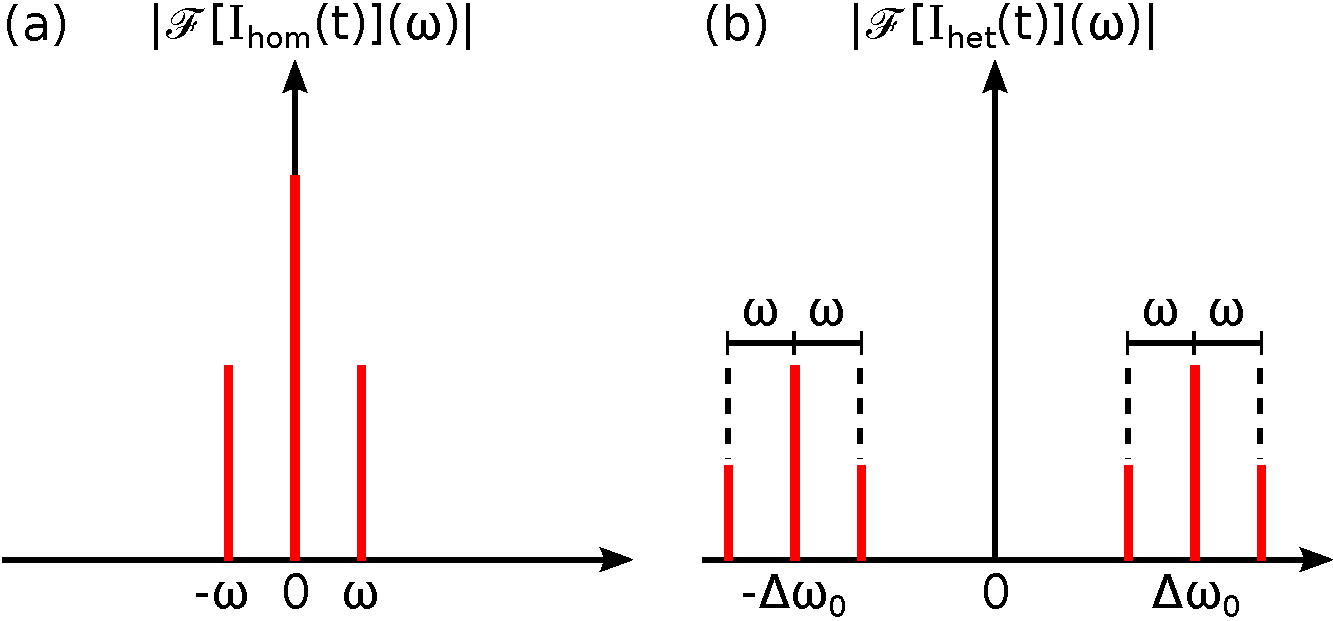
\includegraphics[width = \textwidth]{%
    Chapters/InterferometricMethods/figs/baseband_vs_intermediate_frequency.pdf}
  \caption[Schematic of homodyne vs.\ heterodyne signals in frequency space]{%
    Schematic of (a) homodyne vs.\ (b) heterodyne signals in frequency space.
    A homodyne signal is predominantly DC, and
    a sinusoidal fluctuation with angular frequency $\omega$
    produces sidebands at $\pm \omega$.
    In contrast, the power in a heterodyne signal is shifted
    to the intermediate frequencies $\pm \Delta \omega_0$, and
    a sinusoidal fluctuation with angular frequency $\omega$
    produces sidebands at $\Delta \omega_0 \pm \omega$ and
    $-\Delta \omega_0 \pm \omega$.}
  \label{fig:InterferometricMethods:baseband_vs_intermediate_frequency}
\end{figure}

The heterodyne interference signal must be demodulated
in order to retrieve the baseband phase-fluctuation information.
\graffito{\textcolor{red}{More on demodulation hardware in Ch.~3}}
Practically speaking, dedicated analog or digital electronics
are used to demodulate the heterodyne signal;
however, for the pedagogical purposes of this section,
it is sufficient to consider the ``equivalent optical intensities''
corresponding to the demodulated signals.
The so-called in-phase ($I$) and quadrature ($Q$) signals
are obtained by mixing $I_{\text{het}}$ with
$\real(e^{-i \Delta\omega_0 t})$ and
$\imag(e^{-i \Delta\omega_0 t})$, respectively, and
low-pass filtering the resulting signals;
here, for simplicity, low-pass filtering is implemented
by averaging over a cycle of the intermediate frequency.
Thus, the equivalent $I$ and $Q$ optical intensities are defined as
\begin{align}
  I_{I}(\vect{r}_{\image}, t)
  +
  i \cdot I_{Q}(\vect{r}_{\image}, t)
  &=
  \langle
  e^{-i \Delta \omega_0 t} \cdot I_{\text{het}}(\vect{r}_{\image}, t)
  \rangle_{\Delta \omega_0}
  \notag \\
  &=
  I_G(\vect{r}_{\image})
  e^{i \bar{\phi}}
  \left[ 1 + i \tilde{\phi}(x_{\image}, t) \right],
  \label{eq:InterferometricMethods:heterodyne_interferometer_I_and_Q_intensity}
\end{align}
where $\langle q \rangle_{\Delta \omega_0}$ denotes
the average of quantity $q$ over an intermediate-frequency cycle as
\begin{equation}
  \langle q \rangle_{\Delta \omega_0}
  \equiv
  \frac{\Delta \omega_0}{2 \pi}
  \int_{0}^{\Delta \omega_0 / 2 \pi}
  q(t) dt.
  \label{eq:InterferometricMethods:intermediate_frequency_cycle_average}
\end{equation}

In contrast to the homodyne interferometer,
the heterodyne interferometer makes an absolute measurement
of the phase-fluctuation amplitude $\tilde{\phi}_0$.
To see this, note that $I_{I}$ and $I_{Q}$
(the real and imaginary components of
(\ref{eq:InterferometricMethods:heterodyne_interferometer_I_and_Q_intensity}),
respectively)
can be separated into equilibrium and fluctuating components as
\begin{align}
  \bar{I}_{I}(\vect{r}_{\image}, t)
  &=
  I_G(\vect{r}_{\image}) \cos\bar{\phi},
  \\
  \bar{I}_{Q}(\vect{r}_{\image}, t)
  &=
  I_G(\vect{r}_{\image}) \sin\bar{\phi},
  \\
  \tilde{I}_{I}(\vect{r}_{\image}, t)
  &=
  -I_G(\vect{r}_{\image})
  \sin\bar{\phi}
  \cdot
  \tilde{\phi}(x_{\image}, t),
  \\
  \tilde{I}_{Q}(\vect{r}_{\image}, t)
  &=
  I_G(\vect{r}_{\image})
  \cos\bar{\phi}
  \cdot
  \tilde{\phi}(x_{\image}, t).
\end{align}
As is the case for the homodyne interferometer,
there are three potentially dynamic quantities:
$\{\bar{\phi}, \, \tilde{\phi}(x_{\image}, t), \, I_G(\vect{r}_{\image})\}$;
however, in contrast to the homodyne interferometer,
there are now \emph{four} measured quantities:
$\{\bar{I}_{I}, \, \bar{I}_{Q}, \, \tilde{I}_{I}, \, \tilde{I}_{Q}\}$.
Therefore, the number of measured quantities
is sufficient to unambiguously determine
$\{\bar{\phi}, \, \tilde{\phi}(x_{\image}, t), \, I_G(\vect{r}_{\image})\}$
in absolute units.

Finally, it is useful to characterize
the heterodyne interferometer's performance
relative to the saturation limits of a given detector.
Because $|\tilde{\phi}(x_{\image}, t)| \ll 1$, the heterodyne intensity
(\ref{eq:InterferometricMethods:heterodyne_intensity})
can be approximated as
\begin{align}
  I_{\text{het}}(\vect{r}_{\image}, t)
  &\approx
  2 I_G(\vect{r}_{\image}) [1 + \cos(\Delta \omega_0 t + \bar{\phi})]
  \notag \\
  &\leq
  4 I_G(0),
  \notag
\end{align}
where $I_G(0) = I_G(\rho_{\image} = 0, z_{\image})$ is convenient shorthand
for the peak intensity of the unscattered Gaussian probe beam at the detector.
To obtain optimal performance, select $I_G(0)$ such that
\begin{equation}
  I_{\text{sat}}
  =
  4 I_G(0).
  \notag
\end{equation}
Further, define the total fluctuating intensity
in the demodulated signals to be
\begin{align}
  \left| \tilde{I}_{IQ}(\vect{r}_{\image}, t) \right|
  &\equiv
  \left\{%
    [\tilde{I}_{I}(\vect{r}_{\image}, t)]^2
    +
    [\tilde{I}_{Q}(\vect{r}_{\image}, t)]^2
  \right\}^{1/2}
  \notag \\
  &=
  I_G(\vect{r}_{\image})
  \cdot
  \left| \tilde{\phi}(x_{\image}, t) \right|
  \label{eq:InterferometricMethods:heterodyne_total_fluctuating_intensity}
\end{align}
such that the fraction of the detector's dynamic range
occupied by the fluctuating component in the demodulated signal is
\begin{equation}
  \frac{\left| \tilde{I}_{IQ}(\vect{r}_{\image}, t) \right|}{I_{\text{sat}}}
  =
  \frac{I_G(\vect{r}_{\image})}{I_G(0)}
  \cdot
  T_{\text{het}}
  \cdot
  \left| \tilde{\phi}(x_{\image}, t) \right|,
\end{equation}
where
\begin{equation}
  T_{\text{het}}
  \equiv
  \frac{1}{4}
  \label{eq:InterferometricMethods:heterodyne_interferometer_wavenumber_transfer_function}
\end{equation}
is the heterodyne interferometer's transfer function.
As presented here,
$T_{\text{het}}$ is independent of the fluctuation wavenumber;
however, the finite sampling-volume effects
that accompany any real-world measurement
introduce a wavenumber dependence,
as discussed in
Section~\ref{sec:DesignConsiderations:geometric:finite_sampling_volume}.

In contrast to the homodyne interferometer,
the heterodyne interferometer's wavenumber transfer function
is \emph{not} a function of $\phi_R - \bar{\phi}$.
Thus, the heterodyne interferometer always operates at its peak sensitivity,
regardless of the bulk plasma phase or path-length vibrations.
Robust sensitivity comes at a cost, however.
Note that
\begin{equation}
  \frac{T_{\text{het}}}{T_{\text{hom}}}
  =
  \frac{1}{2}
  \quad
  \text{for homodyne operation at $\phi_R - \bar{\phi} = \pi / 2$.}
  \notag
\end{equation}
Thus, for a given detector,
a heterodyne interferometer will be two times \emph{less} sensitive
than a homodyne interferometer operated in its optimal configuration
($\phi_R - \bar{\phi} = \pi / 2$).
The physical origin of the heterodyne interferometer's sensitivity deficit
is the mixing process used to demodulate
the intermediate-frequency interference signal,
which reduces the signal power by a factor of two
(the rest of the signal power is mixed up
to twice the intermediate frequency and
is removed via low-pass filtering).


\section{Phase contrast imaging (PCI)}
\label{sec:InterferometricMethods:pci}
As discussed in
Section~\ref{sec:InterferometricMethods:imaging:need_for_reference_beam},
imaging the probe radiation on a square-law detector
produces a very weak response
because the unscattered and scattered beams
are $\pi / 2$ out of phase with each other.
To produce a measurable response, a traditional interferometer
interferes the imaged radiation with an external reference beam.
If the phase of the unscattered beam could be manipulated, though,
the external reference beam would no longer be needed.
This is the approach employed in phase contrast imaging (PCI).
A typical PCI system is shown schematically in
Fig.~\ref{fig:InterferometricMethods:pci_schematic}.

\begin{figure}
  \centering
  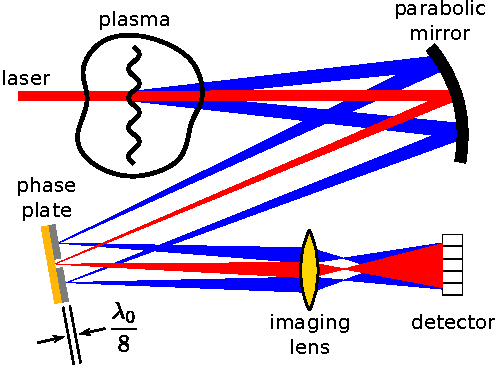
\includegraphics[width = 0.75 \textwidth]{%
    Chapters/InterferometricMethods/figs/pci_schematic.pdf}
  \caption[Schematic overview of a typical PCI system]{%
    Schematic overview of a typical PCI system.
    A plasma-density fluctuation weakly scatters an incident probe beam, and
    an off-axis parabolic mirror focuses the scattered and unscattered beams.
    An optical element known as a phase plate
    is placed at the focal plane of the parabolic mirror.
    The phase plate has a narrow groove of depth $\lambda_0 / 8$
    that imparts phase delay $\pi / 2$ to the unscattered beam,
    effectively converting the unscattered beam
    into an ``internal'' reference beam
    against which the scattered beams can be interfered.
    A lens, whose object plane sits at the plasma midplane,
    is then used to image the resulting radiation onto a detector array.}
  \label{fig:InterferometricMethods:pci_schematic}
\end{figure}


\subsection{Reference-beam generation with a phase plate}
PCI uses an optical element known as a \emph{phase plate}
to delay the unscattered beam by $\pi / 2$
relative to the scattered beams.
The phase plate is typically a reflective optical element
with a groove that is precisely fabricated
to have a depth of $\lambda_0 / 8$;
the unscattered beam reflects off of this groove, and
the corresponding $\lambda_0 / 4$-increase in path length
phase delays the unscattered beam by $\pi / 2$
relative to the scattered beams,
which reflect off of the non-grooved portions
(i.e.\ the ``face'') of the phase plate.
To boost the relative size of the fluctuating signal,
the phase groove typically reflects only a fraction $\eta < 1$
of the incident unscattered beam power, while
the phase-plate face reflects all of the scattered beam power.
Thus, by the action of the phase plate,
$1 \rightarrow i \sqrt{\eta}$ in the imaged electric field
(\ref{eq:InterferometricMethods:imaged_total_field_monochromatic_fluctuation_weak_coupling})
such that
\begin{equation}
  E_{\text{PCI}}(\vect{r}_{\image}, t)
  =
  i E_G(\vect{r}_{\image}, t) e^{i \bar{\phi}}
  \left[%
    \sqrt{\eta} + \tilde{\phi}_0 \cos\nu
  \right],
  \label{eq:InterferometricMethods:pci_imaged_field}
\end{equation}
and the corresponding intensity, to first order in $\tilde{\phi}_0$, is
\begin{equation}
  I_{\text{PCI}}(\vect{r}_{\image}, t)
  =
  I_G(\vect{r}_{\image})
  \left[%
    \eta
    +
    2 \sqrt{\eta} \tilde{\phi}_0 \cos\nu
  \right].
  \label{eq:InterferometricMethods:pci_intensity}
\end{equation}
Here, $E_G(\vect{r}_{\image})$ and $I_G(\vect{r}_{\image})$
are the field and intensity profiles
of the unscattered Gaussian beam on the detector
in the \emph{absence} of the phase plate,
with $I_G(\vect{r}_{\image})$ being explicitly defined in
(\ref{eq:InterferometricMethods:Gaussian_beam_intensity}).
Equation
(\ref{eq:InterferometricMethods:pci_intensity})
should be contrasted with
(\ref{eq:InterferometricMethods:imaged_field_intensity}),
which gives the image-plane intensity
in the absence of the phase plate.
Thus, the phase plate converts the unscattered probe beam
into an effective reference beam for the scattered beams.


\subsection{Focal-plane separation of scattered beams}
Implicit in the use of the phase plate
is that the scattered and unscattered beams
are well-separated in space
such that the phase groove only affects the unscattered beam.
The 1\ts{st}-order scattered beams are angularly separated
from the unscattered beam by $\theta = k / k_0$, and,
in the far field ($z \gg z_R$),
the center of the scattered beam will fall outside of
the unscattered beam's 1/e $E$ radius if
\begin{equation}
  |k| \geq \frac{2}{w_0}.
  \label{eq:InterferometricMethods:kmin_for_far_field_beam_separation}
\end{equation}
However, CO$_2$ laser beams used to probe tokamak plasmas often have
$z_R \gg \SI{10}{\meter}$, so
the beam's far field is not easily accessible in typical lab settings.
Fortunately, the far-field diffraction pattern
can be equivalently accessed in the focal plane
of a focusing optic~\cite[Ch.~8]{born_and_wolf}.

The focal-plane location, beam size, and beam separation
can be easily determined.
Let the Gaussian probe beam have
an in-vessel 1/e $E$ waist radius of $w_0$,
and place a focusing optic of focal length $f$
a distance $s$ downstream from the in-vessel beam waist.
Then, the waist of the focused beam
will be located a distance $s'$ downstream of the focusing optic
and will have 1/e $E$ radius $w_0'$ given as
\begin{align}
  s' &= f \left( 1 + \frac{s - f}{z_R} \right),
  \\
  w_0' &= \frac{w_0 |f|}{\left[ (s - f)^2 + z_R^2 \right]^{1/2}},
\end{align}
where $z_R$ is the in-vessel Rayleigh length~\cite{self83}.
When $|s - f| \ll z_R$, as is typical for PCI,
the expressions for $s'$ and $w_0'$ reduce to
\begin{align}
  s' &\approx f,
  \label{eq:InterferometricMethods:focal_plane_location_rayleigh}
  \\
  w_0' &\approx \frac{2 |f|}{k_0 w_0}.
  \label{eq:InterferometricMethods:focal_plane_waist_rayleigh}
\end{align}
The spatial separation $\Delta$
of the scattered and unscattered beams in the focal plane
is found by applying the appropriate $ABCD$ ray matrices
from Table~\ref{table:ImagingSystems:ABCD_matrices}
to a ray scattered in the plasma midplane by angle $\theta$, i.e.\
\begin{align}
  \begin{pmatrix}
    \Delta
    \\
    \theta_{pp}
  \end{pmatrix}
  &=
  \begin{pmatrix}
    1 & s'
    \\
    0 & 1
  \end{pmatrix}
  \begin{pmatrix}
    1      & 0
    \\
    -1 / f & 1
  \end{pmatrix}
  \begin{pmatrix}
    1 & s
    \\
    0 & 1
  \end{pmatrix}
  \begin{pmatrix}
    0
    \\
    \theta
  \end{pmatrix},
  \notag
\end{align}
which, upon substitution of
of the focal plane location from
(\ref{eq:InterferometricMethods:focal_plane_location_rayleigh}) and
the scattering angle $\theta = k / k_0$,
simplifies to
\begin{equation}
  \Delta
  \approx
  \frac{k f}{k_0}.
  \label{eq:InterferometricMethods:phase_plate_beam_separation}
\end{equation}


\subsection{Low-$k$ cutoff of phase plate}
Now, let the phase-plate groove have a width $d$, as is shown in
Fig.~\ref{fig:InterferometricMethods:phase_plate_beam_separation}.
Finite PCI response requires that (most of) the scattered beams
fall outside of the phase groove (i.e.\ $|\Delta| \geq d / 2$).
Application of the phase-plate beam-separation formula
(\ref{eq:InterferometricMethods:phase_plate_beam_separation})
then shows that there will be finite PCI response
for $|k| \geq k_g$, where
\begin{equation}
  k_g \equiv \frac{k_0 d}{2 f}.
  \label{eq:InterferometricMethods:pci_kmin_engineering}
\end{equation}
Here, the subscript $g$ is in reference
to the \emph{groove} of the phase plate.
Further, to provide the strongest phase contrast,
the unscattered beam should fall wholly within the phase groove
(i.e.\ $2 w_0' \leq d$);
substituting (\ref{eq:InterferometricMethods:focal_plane_waist_rayleigh})
for $w_0'$ then yields a constraint on the phase groove width
\begin{equation}
  d \geq \frac{4 f}{k_0 w_0},
  \label{eq:InterferometricMethods:phase_groove_constraint}
\end{equation}
and inserting (\ref{eq:InterferometricMethods:phase_groove_constraint}) into
(\ref{eq:InterferometricMethods:pci_kmin_engineering}) yields
\begin{equation}
  k_g \geq \frac{2}{w_0}.
  \label{eq:InterferometricMethods:pci_kmin_physics}
\end{equation}
As finite response requires that $|k| \geq k_g$, it follows that
(\ref{eq:InterferometricMethods:pci_kmin_physics}) is equivalent to
(\ref{eq:InterferometricMethods:kmin_for_far_field_beam_separation}),
which was derived by considering the far-field separation
of the scattered and unscattered beams.
Thus, PCI's low-$k$ cutoff
is ultimately constrained by the in-vessel beam size $w_0$,
with diffraction being the constraining physical mechanism.

\begin{figure}
  \centering
  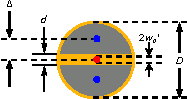
\includegraphics[width = 0.75 \textwidth]{%
    Chapters/InterferometricMethods/figs/phase_plate_beam_separation.pdf}
  \caption[Transverse phase-plate dimensions]{%
    Transverse phase-plate dimensions.
    The unscattered beam is shown in red, while
    the scattered beams are shown in blue.}
  \label{fig:InterferometricMethods:phase_plate_beam_separation}
\end{figure}


\subsection{High-$k$ cutoff of phase plate}
Let the phase plate have a diameter $D$, as is shown in
Fig.~\ref{fig:InterferometricMethods:phase_plate_beam_separation}.
Detection of the scattered radiation
requires that (most of) the scattered beam reflect
from the face of the phase plate
(e.g.\ $\Delta \leq D / 2$).
Application of the phase-plate beam-separation formula
(\ref{eq:InterferometricMethods:phase_plate_beam_separation})
then shows that there will be finite PCI response for $|k| \leq k_D$ where
\begin{equation}
  k_D \equiv \frac{k_0 D}{2 f}.
  \label{eq:InterferometricMethods:pci_kmax_engineering}
\end{equation}


\subsection{Effect of phase plate on $m$\ts{th} scattered beam}
The effect of the PCI phase plate on the $m$\ts{th} scattered beam
is given by the complex-valued function $\mathcal{E}(\vect{r}_m, k)$,
which is derived and thoroughly discussed in
Appendix~\ref{app:PCIResponseIdentities}.
The relevant results are briefly summarized here for completeness.
Eq.~(\ref{eq:PCIResponseIdentities:transformation_Hermitian_decomposed})
shows that PCI's image-plane $\mathcal{E}(\vect{r}_m, k)$
readily reduces to
\begin{equation}
  \begin{aligned}
    \mathcal{E}(\vect{r}_{m,\image}, k_{\image})
    &=
    e^{-[x_{m,\image} / w(z_{m,\image})]^2}
    e^{i m k_{\image} x_{\image}}
    \\
    &\quad\times
    \left[%
      F(\vect{r}_{m,\image}, k_{\image})
      +
      G(\vect{r}_{m,\image}, k_{\image})
    \right],
  \end{aligned}
  \label{eq:InterferometricMethods:PCI_transformation_Hermitian_decomposed}
\end{equation}
where the phase-plate face acts on the $m$\ts{th} scattered beam via $F$, and
the phase-plate groove acts on the $m$\ts{th} scattered beam via $G$.
$F$ and $G$ are themselves defined in
(\ref{eq:PCIResponseIdentities:transformation_face}) and
(\ref{eq:PCIResponseIdentities:transformation_groove}).
Of particular note, $F$ is Hermitian with respect to $m$
\begin{equation}
  F(\vect{r}_{-m,\image}, k_{\image})
  =
  F^*(\vect{r}_{m,\image}, k_{\image}),
  \label{eq:InterferometricMethods:mth_beam_interaction_with_face_hermitian}
\end{equation}
while $G$ is anti-Hermitian with respect to $m$
\begin{equation}
  G(\vect{r}_{-m,\image}, k_{\image})
  =
  -G^*(\vect{r}_{m,\image}, k_{\image}).
  \label{eq:InterferometricMethods:mth_beam_interaction_with_groove_antihermitian}
\end{equation}
These symmetries imply
that $F(\vect{r}_{0,\image}, k_{\image})$ is purely \emph{real} and
that $G(\vect{r}_{0,\image}, k_{\image})$ is purely \emph{imaginary}.


\subsection{The imaged field and its intensity}
\label{sec:InterferometricMethods:pci:imaged_field_and_intensity}
Introducing the notational shorthand
$F_m \equiv F(\vect{r}_{m,\image}, k_{\image})$ and
$G_m \equiv G(\vect{r}_{m,\image}, k_{\image})$,
the weak-coupling ($\tilde{\phi}_0 \ll 1$), image-plane electric field from
(\ref{eq:InterferometricMethods:imaged_total_field_weak_coupling_Fourier_filtered})
readily reduces to
\begin{equation}
  \begin{aligned}
  E(\vect{r}_{\image}, t)
  \approx
  E_G(\vect{r}_{\image}, t)
  e^{i \bar{\phi}}
  \biggl\{%
    F_{0} + G_{0}
    &+
    i \frac{\tilde{\phi}_0}{2}
    \biggl[
      (F_{1} + G_{1}) e^{i \nu}
      \\
      &+
      (F_{-1} + G_{-1}) e^{-i \nu}
    \biggr]
  \biggr\},
  \end{aligned}
\end{equation}
where the approximation $w(z_m) \approx w(z)$ has been used,
$\nu$ is defined in (\ref{eq:InterferometricMethods:image_plane_nu}), and
$E_G(\vect{r}_{\image}, t)$ would be the image-plane electric field
of the unscattered beam in the \emph{absence} of the phase plate.
Now, recall that $F$ is Hermitian such that
$F_{-1} = F^{*}_{1}$ and $F_{0} = \real(F_{0})$ and
that $G$ is anti-Hermitian such that
$G_{-1} = -G^{*}_{1}$ and $G_{0} = {i \cdot \imag(G_{0})}$;
using these substitutions, the field further reduces to
\begin{equation}
  \begin{aligned}
    E(\vect{r}_{\image}, t)
    =
    E_G(\vect{r}_{\image}, t)
    e^{i \bar{\phi}}
    \biggl\{%
      &\real(F_0) - \tilde{\phi}_0 \imag(G_1 e^{i \nu})
      \\
      &+
      i \left[ \imag(G_0) + \tilde{\phi}_0 \real(F_1 e^{i \nu}) \right]
    \biggr\},
  \end{aligned}
\end{equation}
and the corresponding intensity, to first order in $\tilde{\phi}_0$, is
\begin{equation}
  \begin{aligned}
    I_{\text{pci}}(\vect{r}_{\image}, t)
    &=
    I_G(\vect{r}_{\image})
    \biggl\{%
      |F_0|^2 + |G_0|^2
      \\
      &
      +
      2 \tilde{\phi}_0
      \bigl[%
        \imag(G_0) \real(F_1 e^{i \nu})
        -
        \real(F_0) \imag(G_1 e^{i \nu})
      \bigr]
    \biggr\},
  \end{aligned}
\end{equation}
where $I_G(\vect{r}_{\image})$
would be the intensity profile (averaged over an optical cycle)
of the unscattered beam in the \emph{absence} of the phase plate.
Using the fact that $e^{i \nu} = \cos\nu + {i \sin\nu}$,
$F_1 = \real(F_1) + {i \cdot \imag(F_1)}$, and
$G_1 = \real(G_1) + {i \cdot \imag(G_1)}$,
the image-plane intensity further reduces to
\begin{equation}
  \begin{aligned}
    I_{\text{pci}}(\vect{r}_{\image}, t)
    &=
    I_G(\vect{r}_{\image})
    \biggl\{%
      |F_0|^2 + |G_0|^2
      \\
      &+
      2 \tilde{\phi}_0
      \left[ \imag(G_0)\real(F_1) - \real(F_0)\imag(G_1) \right] \cos\nu
      \\
      &-
      2 \tilde{\phi}_0
      \left[ \imag(G_0)\imag(F_1) + \real(F_0)\real(G_1) \right] \sin\nu
    \biggr\}.
  \end{aligned}
  \label{eq:InterferometricMethods:PCI_image_plane_intensity_linear_combination_of_sine_and_cosine}
\end{equation}

Note that the linear combination
$A_I \cos \nu - A_Q \sin \nu$ for real $A_I$, $A_Q$, and $\nu$
can be rewritten as
\begin{align}
  A_I \cos \nu - A_Q \sin \nu
  &=
  A \cos(\nu + \theta),
  \label{eq:InterferometricMethods:linear_combination_of_sine_and_cosine}
\end{align}
where
$A = (A_I^2 + A_Q^2)^{1/2}$,
$\theta = \atantwo(A_Q, A_I)$,
and $\atantwo(A_Q, A_I)$ is the arctangent function of two arguments, which
uses the signs of $A_Q$ and $A_I$ to correctly determine the quadrant
corresponding to a tangent of $A_Q / A_I$.
Note that the notation is mnemonic:
$A_I$ is the amplitude of the ``in-phase'' ($I$) component
(i.e.\ proportional to the image of the assumed
cosine phase fluctuation $\tilde{\phi}(x, t)$ from
(\ref{eq:InterferometricMethods:cosine_phase_fluctuation})), and
$A_Q$ is the amplitude of the corresponding ``quadrature'' ($Q$) component.

As was the case for external reference-beam interferometry,
it is useful to characterize PCI's performance
relative to the saturation limits of a given detector.
Because $\tilde{\phi}_0 \ll 1$,
the PCI optical intensity
(\ref{eq:InterferometricMethods:PCI_image_plane_intensity_linear_combination_of_sine_and_cosine})
satisfies
\begin{align}
  I_{\text{pci}}(\vect{r}_{\image}, t)
  &\lesssim
  I_G(0)
  \left( |F_0|^2 + |G_0|^2 \right),
  \notag
\end{align}
where $I_G(0) = I_G(\rho_{\image} = 0, z_{\image})$ is convenient shorthand
for the peak intensity of the unscattered Gaussian probe beam at the detector
in the \emph{absence} of the phase plate.
To obtain optimal performance, select $I_G(0)$ such that
\begin{equation}
  I_{\text{sat}}
  =
  I_G(0)
  \left( |F_0|^2 + |G_0|^2 \right),
  \notag
\end{equation}
where $I_{\text{sat}}$ is the detector's linear saturation intensity.
Then, taking inspiration from
(\ref{eq:InterferometricMethods:linear_combination_of_sine_and_cosine}),
the image-plane PCI intensity fluctuations from
(\ref{eq:InterferometricMethods:PCI_image_plane_intensity_linear_combination_of_sine_and_cosine})
can be rewritten as
\begin{equation}
  \frac{\tilde{I}_{\text{pci}}(\vect{r}_{\image}, t)}{I_{\text{sat}}}
  =
  \frac{I_G(\vect{r}_{\image})}{I_G(0)}
  \cdot
  A_{\text{pci}}(k_{\image}, x_{\image})
  \cdot
  \tilde{\phi}_0
  \cos\left[ \nu + \theta_{\text{pci}}(k_{\image}, x_{\image}) \right],
\end{equation}
where
\begin{align}
  A_{\text{pci}}(k_{\image}, x_{\image})
  &\equiv
  \frac{2 A(k_{\image}, x_{\image})}{|F_0|^2 + |G_0|^2},
  \label{eq:InterferometricMethods:PCI_wavenumber_transfer_function}
  \\
  \theta_{\text{pci}}(k_{\image}, x_{\image})
  &\equiv
  \atantwo(A_Q, A_I),
\end{align}
and
\begin{align}
  A(k_{\image}, x_{\image})
  &\equiv
  (A_I^2 + A_Q^2)^{1/2},
  \\
  A_I(k_{\image}, x_{\image})
  &\equiv
  \imag(G_0)\real(F_1) - \real(F_0)\imag(G_1),
  \label{eq:InterferometricMethods:PCI_response_AI}
  \\
  A_Q(k_{\image}, x_{\image})
  &\equiv
  \imag(G_0)\imag(F_1) + \real(F_0)\real(G_1).
  \label{eq:InterferometricMethods:PCI_response_AQ}
\end{align}

Thus, the action of the phase plate results in both
an amplitude response $A_{\text{pci}}(k_{\image}, x_{\image})$ and
a phase response $\theta_{\text{pci}}(k_{\image}, x_{\image})$
in PCI's image-plane intensity.
The on-axis responses $A_{\text{pci}}(k_{\image}, x_{\image} = 0)$ and
$\theta_{\text{pci}}(k_{\image}, x_{\image} = 0) = 0$
are consistent with previous derivations at $x_{\image} = 0$,
such as \cite[Eq.~2.141]{coda_phd} and \cite[Eq.~20]{rost_low_k_pci}.
The present work, however, explicitly accounts for
the spatial variation in the amplitude and phase responses
across the face of the detector.
Note that $I_{\text{pci}}$ will be a nonlinear function
of the scattering phase fluctuation $\tilde{\phi}(x, t)$
if there are substantial spatial variations in either
$A_{\text{pci}}$ or $\theta_{\text{pci}}$.
The amplitude and phase responses
can be easily evaluated numerically, and
the results for typical system parameters are shown in
Fig.~\ref{fig:InterferometricMethods:phase_plate_amplitude_and_phase_response}.
As is colloquially understood, the amplitude response
drops precipitously across the full beam profile for $|k| \lesssim k_g$.
(Additionally, the spatial variation in the amplitude response is minimal).
However, perhaps less well known, is the fact that
the phase response varies substantially in space for $|k| \lesssim k_g$.
Thus, PCI's operation for $|k| \lesssim k_g$ is \emph{nonlinear} and
cannot be described in terms of a transfer function;
this can e.g.\ prevent PCI from measuring wavenumbers
of low-$k$ coherent MHD modes, as is discussed in
Section~\ref{sec:InterferometricMethods:selection:pci_low_k_upshift}.
Fortunately, for $|k| \gtrsim k_g$, spatial variations
in $\theta_{\text{pci}}$ are negligible, and,
as a result, PCI's operation is essentially linear and
can be described in terms of a transfer function.

\begin{figure}
  \centering
  \includegraphics[width = \textwidth]{%
    Chapters/InterferometricMethods/figs/phase_plate_amplitude_and_phase_response.pdf}
    \caption[PCI amplitude and phase responses in object-plane coordinates
    ]{%
    PCI amplitude response $A_{\text{pci}}(k, x)$ and
    phase response $\theta_{\text{pci}}(k, x)$
    in object-plane coordinates.
    Spatial coordinates $x$ and wavenumbers $k$ are normalized
    to the 1/e $E$ radius of the in-vessel probe beam, $w_0$.
    The system magnification is $M = 0.5$, a fairly typical value.
    The dashed horizontal lines indicate
    the low-$k$ cutoff of the PCI phase-plate groove, $k_g$;
    here, $k_g = 2 / w_0$,
    which is the minimum value allowed by diffraction,
    as discussed in
    (\ref{eq:InterferometricMethods:pci_kmin_physics}).
    The phase-plate high-$k$ cutoff, $k_D$,
    is taken to be infinite.
    The reflectivity of the phase groove is $\eta = 0.17$,
    which is characteristic of the ZnSe typically
    employed in $\SI{10.6}{\micro\meter}$ optics.
    Note that the low-$k$ phase response $\theta_{\text{pci}}$
    exhibits dramatic spatial variation,
    which results in nonlinear PCI operation for $|k| \lesssim k_g$.
  }
\label{fig:InterferometricMethods:phase_plate_amplitude_and_phase_response}
\end{figure}

As is the case with the homodyne interferometer,
the PCI technique does \emph{not} make an absolute measurement
of the phase-fluctuation amplitude $\tilde{\phi}_0$.
To see this, note that the PCI amplitude response $A_{\text{pci}}$
depends very sensitively on the system alignment,
with slight excursions of the unscattered beam
from the partially reflective phase-plate groove
onto the fully reflective phase-plate face
resulting in macroscopic changes to the power reaching the detector.
Further, power fluctuations at the beam source
can alter $I_G(\vect{r}_{\image})$.
Thus, there are three potentially dynamic quantities:
$\{\tilde{\phi}_0, I_G(\vect{r}_{\image}), A_{\text{pci}}\}$,
but there are only two potentially measurable quantities:
the equilibrium and fluctuating powers.
PCI systems on large, vibration-prone fusion devices
typically employ feedback stabilization
(see e.g.~\cite[Ch.~3.5]{coda_phd})
in order to dynamically maintain
the unscattered beam's alignment
on the phase-plate groove,
minimizing vibrational contamination of the PCI signal.
It is then possible, after measuring a calibration constant,
to \emph{estimate} the phase-fluctuation amplitude $\tilde{\phi}_0$ with PCI.


\section{Selecting an interferometric technique}
\label{sec:InterferometricMethods:selection}
\graffito{\textcolor{red}{Update section: no finite sampling-volume effects}}
Sections~\ref{sec:InterferometricMethods:interferometry}
and~\ref{sec:InterferometricMethods:pci}
detail external reference-beam interferometry and
phase contrast imaging (PCI), respectively.
The intent of this section is to synthesize these results and
to discuss the strengths and limitations
of these interferometric techniques
so that a suitable method can be selected for a given application.


% \subsection{A note on notation}
% The transfer functions derived in the preceding sections
% are all written in terms of image-plane wavenumbers $k_{\image}$ and
% image-plane coordinates $x_{\image}$.
% However, one is often interested in the object-plane wavenumbers $k$,
% as they are directly tied to the underlying physics.
% In contrast, image-plane coordinates $x_{\image}$
% emphasize the importance of the detector dimensions
% on the measured interference signal.
% For these reasons, the below discussions
% use transfer functions with the ``hybrid'' parametrization of
% object-plane wavenumbers $k$ and image-plane coordinates $x_{\image}$.
% If the reader favors a different parametrization, however,
% the transformations between the image-plane and object-plane quantities
% are very simple:
% \begin{align}
%   k_{\image} &= \frac{k}{M},
%   \\
%   x_{\image} &= M x_{\object},
% \end{align}
% where $M$ is the imaging system's magnification.


\subsection{Sensitivity}
The amplitude of the fluctuating signal at the detector
is one of the two aspects
that determines an interferometric system's
signal-to-noise ratio ($\snr$;
the other aspect is the detector noise).
Transfer functions for each interferometric method
were defined in the previous sections
by normalizing the intensity of the fluctuating signal
to the saturation intensity $I_{\text{sat}}$ of a given detector.
Assuming the detectors for each interferometric method
have the same $I_{\text{sat}}$,
a true ``apples-to-apples'' comparison
of signal amplitudes can be made
by examining the amplitudes of the corresponding transfer functions.
Just such a comparison is shown in
Fig.~\ref{fig:InterferometricMethods:interferometric_method_transfer_functions}.
To facilitate the comparison,
the magnification $|M|$ is taken to be the same for each system.

\begin{figure}
  \centering
  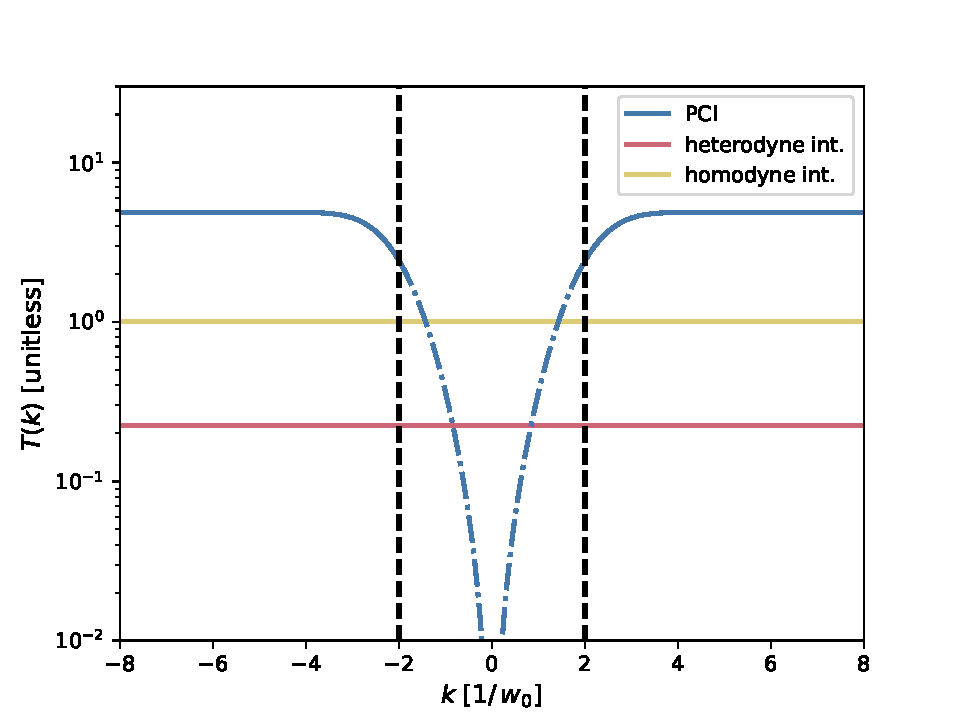
\includegraphics[width = \textwidth]{%
    Chapters/InterferometricMethods/figs/interferometric_method_comparison.pdf}
  \caption[Comparison of interferometric method transfer functions]{%
    A comparison of the PCI amplitude response
    (\ref{eq:InterferometricMethods:PCI_wavenumber_transfer_function})
    to the transfer functions for heterodyne interferometry
    (\ref{eq:InterferometricMethods:heterodyne_interferometer_wavenumber_transfer_function}),
    and homodyne interferometry
    (\ref{eq:InterferometricMethods:homodyne_interferometer_wavenumber_transfer_function},
    in the optimal configuration with $\phi_R - \bar{\phi} = \pi / 2$).
    Object-plane wavenumbers $k$ are normalized
    to the 1/e $E$ radius of the in-vessel probe beam, $w_0$.
    The magnification of each system is taken to be $|M| = 0.5$,
    which is a representative ``typical'' value.
    The vertical, dashed lines indicate
    the low-$k$ cutoff of the PCI phase-plate groove, $k_g$;
    here, $k_g = 2 / w_0$,
    which is the minimum value allowed by diffraction,
    as discussed in
    (\ref{eq:InterferometricMethods:pci_kmin_physics}).
    The phase-plate high-$k$ cutoff, $k_D$,
    is taken to be infinite.
    The reflectivity of the PCI phase groove is $\eta = 0.17$,
    which is characteristic of the ZnSe typically
    employed in $\SI{10.6}{\micro\meter}$ optics.
  }
\label{fig:InterferometricMethods:interferometric_method_transfer_functions}
\end{figure}

Clearly, for a given fluctuation ($|k| \gtrsim k_g$) and detector,
PCI produces a fluctuating signal with the largest amplitude.
Relative to the optimally operating homodyne interferometer
($\phi_R - \bar{\phi} = \pi / 2$),
the PCI's larger amplitude is wholly attributable
to the partial reflectivity ($\eta < 1$) of the phase-plate groove:
the decreased power in the unscattered beam
increases the ratio of fluctuating power to equilibrium power
at the PCI detector.
PCI's sensitivity comes with several costs, however.
First, PCI can only measure phase fluctuations,
whereas external reference-beam interferometers
can measure both equilibrium and fluctuating phase.
This makes intuitive sense:
the equilibrium phase uniformly affects
both the scattered and unscattered beams,
the PCI phase delays the unscattered beam
to generate an ``internal'' reference beam, and
the equilibrium phase information cancels in the resulting interference.
Second, PCI depends very sensitively on the system alignment, and
feedback stabilization is often needed
in order to dynamically maintain
the unscattered beam's alignment on the phase-plate groove
(see e.g.~\cite[Ch.~3.5]{coda_phd}).
While this is an added technical complication,
it should be noted that such feedback stabilization
is expected to become more commonplace
for laser diagnostics on large fusion devices,
such as ITER's heterodyne interferometer
\cite{vanzeeland_TIP_rsi13}.
Finally, as was previously discussed,
PCI does not measure the absolute scale of phase fluctuations, but
calibrations can allow estimates of the absolute scale.

The merits and limitations of homodyne and heterodyne interferometry
were discussed at length in
Sec.~{\ref{sec:InterferometricMethods:interferometry}}, but
they are briefly reviewed here for ease of reference.
The homodyne interferometer's transfer function depends on
the difference between the reference-arm phase and
the equilibrium phase, $\phi_R - \bar{\phi}$,
with peak sensitivity when
$\phi_R - \bar{\phi} = \pi / 2$.
However, due to evolution of the equilibrium phase and vibrations,
it is typically difficult to keep $\phi_R - \bar{\phi}$ fixed at $\pi / 2$.
On small fusion devices,
actively controlled mirrors have been used in an attempt
to account for the evolution of the equilibrium phase and
to cancel vibrational path-length changes,
minimizing excursions from $\phi_R - \bar{\phi} \approx \pi / 2$
\cite{nazikian_rsi87}, but
such an approach has not found application on larger
(and presumably more vibration-prone) fusion experiments.
In contrast, the heterodyne interferometer's transfer function
is independent of $\phi_R - \bar{\phi}$.
Further, in contrast to PCI and homodyne interferometry,
the heterodyne interferometer measures
the absolute scale of phase fluctuations,
independent of any calibration constants.
This robust sensitivity and ability to measure absolute phase fluctuations
comes at a cost, however:
a heterodyne interferometer is four times \emph{less} sensitive
than a homodyne interferometer operated in its optimal configuration
($\phi_R - \bar{\phi} = \pi / 2$), which results from
the need to capture the full sinusoidal waveform
of the heterodyne signal at the detector and
the subsequent need to demodulate the heterodyne signal.


\subsection{Spatial bandwidth}
The spatial bandwidth of both homodyne and heterodyne interferometry
is dictated by the system magnification $M$ and
the detector element's length $s_x$;
these parameters give the finite sampling-volume cutoff,
$k_{\text{fsv}} = 2 \pi M / s_x$.
Finite sampling-volume effects also influence PCI's spatial bandwidth.
While $k_{\text{fsv}}$ was specified to be the same
for all of the interferometric systems displayed in
Fig.~\ref{fig:InterferometricMethods:interferometric_method_transfer_functions},
one could easily imagine altering
a given system's magnification $M$ or detector-element size $s_x$
in order to expand or contract the system's spatial bandwidth.

In addition to finite sampling-volume effects,
PCI's spatial bandwidth is also influenced by
the phase plate's low-$k$ and high-$k$ cutoffs,
$k_g$ and $k_D$, respectively.
The effects of $k_g$, $k_D$, and $k_{\text{fsv}}$
are characterized in
Fig.~\ref{fig:InterferometricMethods:pci_cutoffs}.
The most significant effect of the phase plate
on the spatial bandwidth of the PCI
is to introduce a ``hole'' in the low-$k$ response of the system;
external reference-beam interferometers, in contrast,
do not suffer from such a low-$k$ cutoff.
As discussed in
Sec.~\ref{sec:InterferometricMethods:pci:imaged_field_and_intensity},
the PCI also operates nonlinearly in this low-$k$ ``hole'';
one consequence of this nonlinear operation is discussed in
Sec.~\ref{sec:InterferometricMethods:selection:pci_low_k_upshift}.

\begin{figure}
  \centering
  \includegraphics[width = \textwidth]{%
    Chapters/InterferometricMethods/figs/pci_cutoffs.pdf}
  \caption[Effects of phase-plate and finite sampling-volume cutoffs
      on the PCI transfer function]{%
    Effects of the low-$k$ ($k_g$) and high-$k$ ($k_D$) phase-plate cutoffs
    on the phase-plate transfer function, $T_{\text{pp}}(k)$;
    inclusion of finite sampling-volume effects
    then yields the full PCI transfer function, $T_{\text{pci}}(k)$.
    Object-plane wavenumbers $k$ are normalized
    to the 1/e $E$ radius of the in-vessel probe beam, $w_0$.
    The vertical, dashed lines indicate
    the low-$k$ cutoff of the PCI phase-plate groove, $k_g$;
    here, $k_g = 2 / w_0$,
    which is the minimum value allowed by diffraction,
    as discussed in
    (\ref{eq:InterferometricMethods:pci_kmin_physics}).
    The vertical, dashed-dotted lines indicate
    the phase-plate's high-$k$ cutoff,
    chosen here to be $k_D = 20 / w_0$.
    The finite sampling-volume cutoff $k_{\text{fsv}} = 30 / w_0$
    results from representative ``typical'' values of
    system magnification $|M| = 0.5$ and
    detector-element size $s_x \approx 0.105 w_0$.
    Note that here $k_D < k_{\text{fsv}}$, in contrast to
    Fig.~\ref{fig:InterferometricMethods:interferometric_method_transfer_functions}.
    The reflectivity of the PCI phase groove is $\eta = 0.17$,
    which is characteristic of the ZnSe typically
    employed in $\SI{10.6}{\micro\meter}$ optics.
    As discussed in
    Section~\ref{sec:InterferometricMethods:pci:imaged_field_and_intensity},
    $T_{\text{pp}}$ and $T_{\text{pci}}$ are only true transfer functions
    for $|k| \gtrsim 2 k_g$;
    for smaller wavenumbers, the PCI phase response
    varies significantly across the beam profile,
    resulting in nonlinear operation.
    Regardless, the corresponding ``transfer functions'' are plotted
    across the full $k$-range here and
    correspond to the beam center ($x = 0$).
  }
\label{fig:InterferometricMethods:pci_cutoffs}
\end{figure}

Finally, it should be noted that the above transfer functions
have all been computed assuming that the beams are \emph{not} clipped
by apertures in their corresponding optical trains.
Aperture diffraction minimally affects Gaussian beam propagation if
\begin{equation}
  a_{\text{eff}} \geq \frac{3}{2} w(z),
  \label{eq:InterferometricMethods:aperture_radius_for_minimal_diffraction}
\end{equation}
where $a_{\text{eff}}$ is the effective aperture radius and
$w(z)$ is the beam's 1/e $E$ radius at the location of the aperture
\cite{campbell_josa69, rost_diffraction_pc14}.


\subsection{Nonlinear upshift in low-$k$, PCI-measured wavenumber}
\label{sec:InterferometricMethods:selection:pci_low_k_upshift}
This section discusses a little-known diagnostic artifact of the PCI
that becomes relevant when the fluctuation wavenumber
is smaller than the PCI's low-$k$ cutoff (i.e.\ $|k| \lesssim k_g$).
This effect can be important when trying to measure the wavenumber of
e.g.\ low-$k$ coherent MHD modes, and
it results from PCI's nonlinear operation for $|k| \lesssim k_g$,
which is thoroughly discussed in
Section~\ref{sec:InterferometricMethods:pci:imaged_field_and_intensity}.

It is easiest to see the effects of PCI's nonlinear low-$k$ operation
by defining the normalized fluctuating power
$\tilde{p}_j(t)$
\begin{align}
  \tilde{p}_j(t)
  &=
  \frac{I_G(0)}{I_G(\vect{r}_{\image,j})}
  \cdot
  \frac{1}{\tilde{\phi}_0 |T_{\text{pci}}(k_{\image}, x_{\image, j})|}
  \left[ \frac{\tilde{P}_{j, \, \text{pci}}(t)}{P_{\text{sat}}} \right]
  \notag \\
  &=
  \cos\left[ \nu_j + \theta(k_{\image}, x_{\image, j}) \right].
\end{align}
(This choice of normalization becomes readily apparent after referencing
(\ref{eq:InterferometricMethods:PCI_ratio_fluctuating_to_equilibrium_power})).
The set of measurements $\{\tilde{p}_j(t)\}$
can be e.g.\ Fourier analyzed in the spatial dimension
to provide an estimate of the corresponding
wavenumber autospectral density
$G_{\tilde{p}\tilde{p}}(k_{\text{meas}}, t)$.
\graffito{\textcolor{red}{more details on $G_{xx}(k)$ in Ch.~4}}
When PCI operates linearly,
the measured wavenumber spectrum
has a peak at $k_{\text{meas}} = k$,
with $k$ corresponding to the true, physical wavenumber.
As shown in Fig.~\ref{fig:InterferometricMethods:pci_wavenumber_upshift},
PCI operates linearly for $k \gtrsim k_g$,
as the measured wavenumber spectrum peaks at $k_{\text{meas}} = k$;
however, for $k \lesssim k_g$,
the measured wavenumber spectrum peaks at $k_{\text{meas}} = k_g$,
regardless of the actual fluctuation wavenumber.
The explanation for this effect is relatively simple:
a Gaussian beam can be decomposed into a set of infinite plane waves
traveling in slightly different directions \cite[Ch.~16.7]{siegman_lasers},
and only the components of the scattered beam
with transverse lab-frame wavenumbers $k \geq k_g$
are reflected from the phase-plate face and
produce measurable interference on the PCI detector.
Thus, when $|k| \lesssim k_g$,
not only does the PCI signal's amplitude drop precipitously, but
its spatial content also becomes a nonlinear function
of the corresponding fluctuation wavenumber,
destroying any hopes of wavenumber measurement.

\begin{figure}
  \centering
  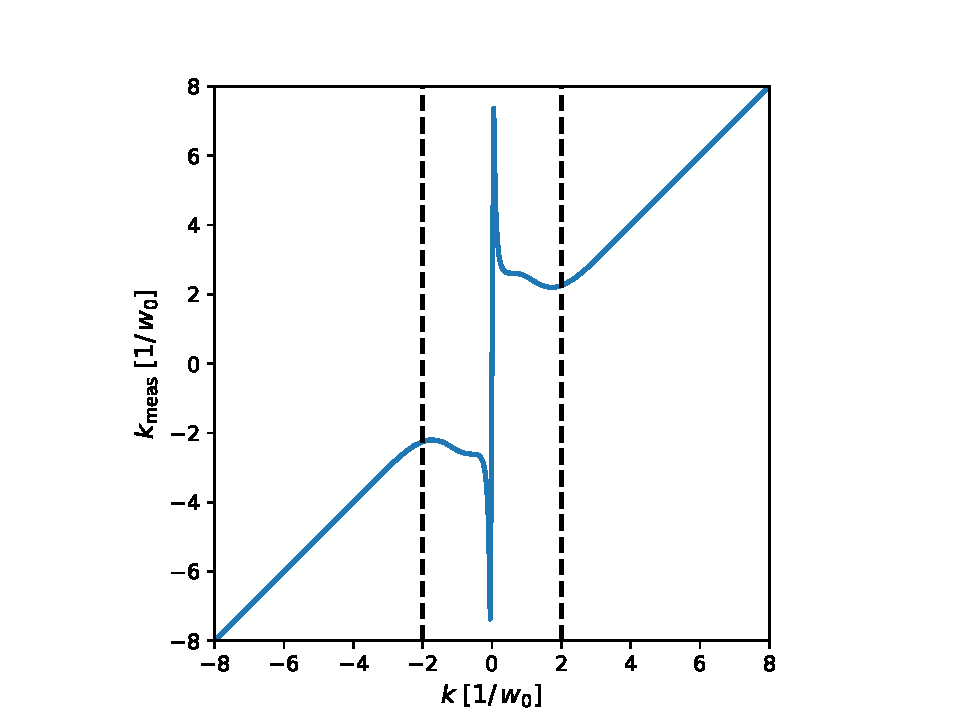
\includegraphics[width = \textwidth]{%
    Chapters/InterferometricMethods/figs/pci_wavenumber_upshift.pdf}
    \caption[Nonlinear upshift in low-$k$, PCI-measured wavenumber]{%
    Estimate of wavenumber autospectral density $G_{\tilde{p}\tilde{p}}(k)$
    that results from Fourier analyzing
    the normalized PCI signal $\tilde{p}$ in space.
    The $y$-axis displays the fluctuation's actual wavenumber $k$, while
    the $x$-axis displays the corresponding ``measured'' wavenumber
    $k_{\text{meas}}$ that results from the Fourier analysis.
    Wavenumbers are all normalized
    to the 1/e $E$ radius of the in-vessel probe beam, $w_0$.
    The horizontal, dashed line indicates
    the low-$k$ cutoff of the PCI phase-plate groove, $k_g$;
    here, $k_g = 2 / w_0$,
    which is the minimum value allowed by diffraction,
    as discussed in
    (\ref{eq:InterferometricMethods:pci_kmin_physics}).
    The system magnification has
    a representative ``typical'' value $|M| = 0.5$.
    Note that PCI operates linearly for $k \gtrsim k_g$,
    as the measured wavenumber spectrum peaks at $k_{\text{meas}} = k$;
    however, for $k \lesssim k_g$,
    the measured wavenumber spectrum peaks at $k_{\text{meas}} = k_g$,
    regardless of the actual fluctuation wavenumber.
  }
\label{fig:InterferometricMethods:pci_wavenumber_upshift}
\end{figure}


\subsection{Temporal bandwidth}
Finally, the required temporal bandwidth should also be considered.
For heterodyne interferometry,
proper reconstruction of the fluctuating baseband signal
at angular frequency $\omega$
from the heterodyne signal
at angular intermediate frequency $\Delta \omega_0$ requires that
$\omega < \Delta \omega_0$.
Further, the detector's angular cutoff frequency $\omega_{\text{det}}$
should be sufficiently large to capture the relevant dynamics such that
\begin{equation}
  \omega_{\text{det}} > \Delta \omega_0 + \omega,
  \qquad
  \text{heterodyne interferometry.}
\end{equation}
In contrast, homodyne interferometry and PCI only require that
\begin{equation}
  \omega_{\text{det}} > \omega,
  \qquad \qquad \quad% \qquad
  \text{homodyne interferometry, PCI.}
\end{equation}
Thus, heterodyne interferometry requires a faster detector
than homodyne interferometry or PCI\@.
For the HgCdTe detectors typically used at $\SI{10.6}{\micro\meter}$,
cooling the active element of the detector
reduces detector noise and increases the detector response
but also reduces $\omega_{\text{det}}$.
Thus, for low-temporal-bandwidth applications,
homodyne interferometry and PCI can use
slower, cooled detectors that will improve
system signal-to-noise ratio ($\snr$)
relative to the faster, warmer detectors
required for heterodyne interferometry.
Deployment of homodyne interferometry or PCI
in high-temporal-bandwidth applications, however,
requires the use of higher bandwidth detectors and/or
more exotic detection techniques, such as
optical heterodyning~\cite[Sec.~3.3.1]{tsujii_phd}.


\bibliographystyle{plainurl}
\bibliography{references}
